\documentclass[twoside]{book}

% Packages required by doxygen
\usepackage{fixltx2e}
\usepackage{calc}
\usepackage{doxygen}
\usepackage[export]{adjustbox} % also loads graphicx
\usepackage{graphicx}
\usepackage[utf8]{inputenc}
\usepackage{makeidx}
\usepackage{multicol}
\usepackage{multirow}
\PassOptionsToPackage{warn}{textcomp}
\usepackage{textcomp}
\usepackage[nointegrals]{wasysym}
\usepackage[table]{xcolor}

% Font selection
\usepackage[T1]{fontenc}
\usepackage[scaled=.90]{helvet}
\usepackage{courier}
\usepackage{amssymb}
\usepackage{sectsty}
\renewcommand{\familydefault}{\sfdefault}
\allsectionsfont{%
  \fontseries{bc}\selectfont%
  \color{darkgray}%
}
\renewcommand{\DoxyLabelFont}{%
  \fontseries{bc}\selectfont%
  \color{darkgray}%
}
\newcommand{\+}{\discretionary{\mbox{\scriptsize$\hookleftarrow$}}{}{}}

% Page & text layout
\usepackage{geometry}
\geometry{%
  a4paper,%
  top=2.5cm,%
  bottom=2.5cm,%
  left=2.5cm,%
  right=2.5cm%
}
\tolerance=750
\hfuzz=15pt
\hbadness=750
\setlength{\emergencystretch}{15pt}
\setlength{\parindent}{0cm}
\setlength{\parskip}{3ex plus 2ex minus 2ex}
\makeatletter
\renewcommand{\paragraph}{%
  \@startsection{paragraph}{4}{0ex}{-1.0ex}{1.0ex}{%
    \normalfont\normalsize\bfseries\SS@parafont%
  }%
}
\renewcommand{\subparagraph}{%
  \@startsection{subparagraph}{5}{0ex}{-1.0ex}{1.0ex}{%
    \normalfont\normalsize\bfseries\SS@subparafont%
  }%
}
\makeatother

% Headers & footers
\usepackage{fancyhdr}
\pagestyle{fancyplain}
\fancyhead[LE]{\fancyplain{}{\bfseries\thepage}}
\fancyhead[CE]{\fancyplain{}{}}
\fancyhead[RE]{\fancyplain{}{\bfseries\leftmark}}
\fancyhead[LO]{\fancyplain{}{\bfseries\rightmark}}
\fancyhead[CO]{\fancyplain{}{}}
\fancyhead[RO]{\fancyplain{}{\bfseries\thepage}}
\fancyfoot[LE]{\fancyplain{}{}}
\fancyfoot[CE]{\fancyplain{}{}}
\fancyfoot[RE]{\fancyplain{}{\bfseries\scriptsize Generated by Doxygen }}
\fancyfoot[LO]{\fancyplain{}{\bfseries\scriptsize Generated by Doxygen }}
\fancyfoot[CO]{\fancyplain{}{}}
\fancyfoot[RO]{\fancyplain{}{}}
\renewcommand{\footrulewidth}{0.4pt}
\renewcommand{\chaptermark}[1]{%
  \markboth{#1}{}%
}
\renewcommand{\sectionmark}[1]{%
  \markright{\thesection\ #1}%
}

% Indices & bibliography
\usepackage{natbib}
\usepackage[titles]{tocloft}
\setcounter{tocdepth}{3}
\setcounter{secnumdepth}{5}
\makeindex

% Hyperlinks (required, but should be loaded last)
\usepackage{ifpdf}
\ifpdf
  \usepackage[pdftex,pagebackref=true]{hyperref}
\else
  \usepackage[ps2pdf,pagebackref=true]{hyperref}
\fi
\hypersetup{%
  colorlinks=true,%
  linkcolor=blue,%
  citecolor=blue,%
  unicode%
}

% Custom commands
\newcommand{\clearemptydoublepage}{%
  \newpage{\pagestyle{empty}\cleardoublepage}%
}

\usepackage{caption}
\captionsetup{labelsep=space,justification=centering,font={bf},singlelinecheck=off,skip=4pt,position=top}

%===== C O N T E N T S =====

\begin{document}

% Titlepage & ToC
\hypersetup{pageanchor=false,
             bookmarksnumbered=true,
             pdfencoding=unicode
            }
\pagenumbering{roman}
\begin{titlepage}
\vspace*{7cm}
\begin{center}%
{\Large rpg tools (Python) \\[1ex]\large 1.\+0a }\\
\vspace*{1cm}
{\large Generated by Doxygen 1.8.11}\\
\end{center}
\end{titlepage}
\clearemptydoublepage
\tableofcontents
\clearemptydoublepage
\pagenumbering{arabic}
\hypersetup{pageanchor=true}

%--- Begin generated contents ---
\chapter{Todo List}
\label{todo}
\hypertarget{todo}{}

\begin{DoxyRefList}
\item[\label{todo__todo000001}%
\Hypertarget{todo__todo000001}%
File \mbox{\hyperlink{backpack_8py}{backpack.py}} ]Todo list
\begin{DoxyItemize}
\item userinterface
\item usermanagment
\item inventorymanagement
\item export 
\end{DoxyItemize}
\end{DoxyRefList}
\chapter{Bug List}
\label{bug}
\hypertarget{bug}{}

\begin{DoxyRefList}
\item[\label{bug__bug000001}%
\hypertarget{bug__bug000001}{}%
Global \hyperlink{globaltools_8py_a388d233340dff99be67f0afc03953992}{rpgtoolbox\+:\+:globaltools.find\+Loops} (struc=\{\}, elem=\textquotesingle{}\textquotesingle{}, way=\mbox{[}\mbox{]}, result=\mbox{[}\mbox{]})]this function finds sometimes loops where no loops are... it seems to concern multiple links to leaves... 
\end{DoxyRefList}
\chapter{Namespace Index}
\section{Packages}
Here are the packages with brief descriptions (if available)\+:\begin{DoxyCompactList}
\item\contentsline{section}{\mbox{\hyperlink{namespacegui_1_1window}{gui.\+window}} \\*Some classes for G\+UI }{\pageref{namespacegui_1_1window}}{}
\end{DoxyCompactList}

\chapter{Hierarchical Index}
\section{Class Hierarchy}
This inheritance list is sorted roughly, but not completely, alphabetically\+:\begin{DoxyCompactList}
\item \contentsline{section}{Auto\+Scrollbar}{\pageref{classgui_1_1winhelper_1_1AutoScrollbar}}{}
\item \contentsline{section}{blank\+Window}{\pageref{classgui_1_1window_1_1blankWindow}}{}
\begin{DoxyCompactList}
\item \contentsline{section}{conf\+Window}{\pageref{classcalc__ep_1_1confWindow}}{}
\item \contentsline{section}{input\+Win}{\pageref{classcalc__ep_1_1inputWin}}{}
\item \contentsline{section}{Main\+Window}{\pageref{classcalc__ep_1_1MainWindow}}{}
\item \contentsline{section}{conf\+Window}{\pageref{classgui_1_1window_1_1confWindow}}{}
\item \contentsline{section}{input\+Win}{\pageref{classgui_1_1window_1_1inputWin}}{}
\item \contentsline{section}{Main\+Window}{\pageref{classgui_1_1window_1_1MainWindow}}{}
\item \contentsline{section}{meta\+Win}{\pageref{classgui_1_1window_1_1metaWin}}{}
\end{DoxyCompactList}
\item \contentsline{section}{chk\+Cfg}{\pageref{classrpgtoolbox_1_1confbox_1_1chkCfg}}{}
\item \contentsline{section}{ep\+Sheet}{\pageref{classcalc__ep_1_1epSheet}}{}
\item \contentsline{section}{Info\+Canvas}{\pageref{classgui_1_1winhelper_1_1InfoCanvas}}{}
\item \contentsline{section}{Magic}{\pageref{classrpgToolDefinitions_1_1MERSTables_1_1Magic}}{}
\item \contentsline{section}{message\+Window}{\pageref{classgui_1_1window_1_1messageWindow}}{}
\item \contentsline{section}{My\+Class}{\pageref{classrpgToolDefinitions_1_1RMTables_1_1MyClass}}{}
\item \contentsline{section}{raised\+Error}{\pageref{classrpgtoolbox_1_1errbox_1_1raisedError}}{}
\end{DoxyCompactList}

\chapter{Data Structure Index}
\section{Data Structures}
Here are the data structures with brief descriptions\+:\begin{DoxyCompactList}
\item\contentsline{section}{\mbox{\hyperlink{classbackpack_1_1src_1_1gui_1_1Tests_1_1Test2_1_1mainwindow}{mainwindow}} \\*Classdocs }{\pageref{classbackpack_1_1src_1_1gui_1_1Tests_1_1Test2_1_1mainwindow}}{}
\item\contentsline{section}{\mbox{\hyperlink{classbackpack_1_1src_1_1gui_1_1window_1_1blankWindow}{blank\+Window}} \\*A simple window class with a not filled menu bar }{\pageref{classbackpack_1_1src_1_1gui_1_1window_1_1blankWindow}}{}
\item\contentsline{section}{\mbox{\hyperlink{classbackpack_1_1src_1_1gui_1_1window_1_1messageWindow}{message\+Window}} \\*A class to build a message window containing version, author and email on default }{\pageref{classbackpack_1_1src_1_1gui_1_1window_1_1messageWindow}}{}
\end{DoxyCompactList}

\chapter{File Index}
\section{File List}
Here is a list of all documented files with brief descriptions\+:\begin{DoxyCompactList}
\item\contentsline{section}{\hyperlink{Backpack_8py}{Backpack.\+py} \\*This is a simple tool to keep track of a character\textquotesingle{}s backpack }{\pageref{Backpack_8py}}{}
\item\contentsline{section}{\hyperlink{calc__ep_8py}{calc\+\_\+ep.\+py} }{\pageref{calc__ep_8py}}{}
\item\contentsline{section}{\hyperlink{confbox_8py}{confbox.\+py} \\*A toolbox of things to handle config files }{\pageref{confbox_8py}}{}
\item\contentsline{section}{\hyperlink{epcalcdefs_8py}{epcalcdefs.\+py} }{\pageref{epcalcdefs_8py}}{}
\item\contentsline{section}{\hyperlink{errbox_8py}{errbox.\+py} \\*A box full of error classes }{\pageref{errbox_8py}}{}
\item\contentsline{section}{\hyperlink{globaltools_8py}{globaltools.\+py} \\*Bunch of nice global tools }{\pageref{globaltools_8py}}{}
\item\contentsline{section}{\hyperlink{helptools_8py}{helptools.\+py} }{\pageref{helptools_8py}}{}
\item\contentsline{section}{\hyperlink{itemshop_8py}{itemshop.\+py} \\*Buying tool for character\textquotesingle{}s equipment }{\pageref{itemshop_8py}}{}
\item\contentsline{section}{\hyperlink{logbox_8py}{logbox.\+py} \\*Module with logging tools }{\pageref{logbox_8py}}{}
\item\contentsline{section}{\hyperlink{MERSTables_8py}{M\+E\+R\+S\+Tables.\+py} \\*Package for Handling M\+E\+R\+S/\+M\+E\+RP tables }{\pageref{MERSTables_8py}}{}
\item\contentsline{section}{\hyperlink{rpgtools_8py}{rpgtools.\+py} }{\pageref{rpgtools_8py}}{}
\item\contentsline{section}{\hyperlink{window_8py}{window.\+py} }{\pageref{window_8py}}{}
\item\contentsline{section}{\hyperlink{winhelper_8py}{winhelper.\+py} \\*Collection of helper tools for building Tk() windows/apps }{\pageref{winhelper_8py}}{}
\end{DoxyCompactList}

\chapter{Namespace Documentation}
\hypertarget{namespacecalc__ep}{}\section{calc\+\_\+ep Namespace Reference}
\label{namespacecalc__ep}\index{calc\+\_\+ep@{calc\+\_\+ep}}


This is a little tool for calculating E\+Ps for M\+E\+R\+S/\+RM.  


\subsection*{Data Structures}
\begin{DoxyCompactItemize}
\item 
class \hyperlink{classcalc__ep_1_1confWindow}{conf\+Window}
\begin{DoxyCompactList}\small\item\em This class builds a window for selecting and saving options of A\+Da\+ManT. \end{DoxyCompactList}\item 
class \hyperlink{classcalc__ep_1_1epSheet}{ep\+Sheet}
\begin{DoxyCompactList}\small\item\em Class for calculating EP sheets. \end{DoxyCompactList}\item 
class \hyperlink{classcalc__ep_1_1inputWin}{input\+Win}
\begin{DoxyCompactList}\small\item\em Objects of this class type are windows for input the wanted data structure. \end{DoxyCompactList}\item 
class \hyperlink{classcalc__ep_1_1MainWindow}{Main\+Window}
\begin{DoxyCompactList}\small\item\em This is the class for the main window object. \end{DoxyCompactList}\end{DoxyCompactItemize}


\subsection{Detailed Description}
This is a little tool for calculating E\+Ps for M\+E\+R\+S/\+RM. 

\begin{DoxyDate}{Date}
(C) 2015-\/2016 
\end{DoxyDate}
\begin{DoxyAuthor}{Author}
Marcus Schwamberger  \href{mailto:marcus@lederzeug.de}{\tt marcus@lederzeug.\+de}  G\+NU V3.\+0 
\end{DoxyAuthor}
\begin{DoxyVersion}{Version}
0.\+3
\end{DoxyVersion}
\begin{DoxyRefDesc}{Todo}
\item[\hyperlink{todo__todo000002}{Todo}]design edit window\+: Critical Hits 

design edit window\+: Killed Monsters 

design edit window\+: used spells 

design\+: enter/save/load character list/party 

design\+: successful maneuvers 

design\+: traveled distance 

design\+: individual E\+Ps\end{DoxyRefDesc}


import Config\+Parser as CP 
\hypertarget{namespacegui}{}\section{gui Namespace Reference}
\label{namespacegui}\index{gui@{gui}}


Classes and stuff for the G\+UI.  


\subsection*{Namespaces}
\begin{DoxyCompactItemize}
\item 
 \hyperlink{namespacegui_1_1window}{window}
\end{DoxyCompactItemize}
\subsection*{Functions}
\begin{DoxyCompactItemize}
\item 
def \hyperlink{namespacegui_a37b31e71da0c76180282154d702cfecb}{check\+Version} ()
\begin{DoxyCompactList}\small\item\em This function checks out the installed (and used) Python version. \end{DoxyCompactList}\end{DoxyCompactItemize}


\subsection{Detailed Description}
Classes and stuff for the G\+UI. 

this toolbox consist of functions and classes for creating a G\+UI. They are used by the main module.

\begin{DoxyAuthor}{Author}
Marcus Schwamberger  \href{mailto:mongol@nld.ds}{\tt mongol@nld.\+ds} mpg.\+de 
\end{DoxyAuthor}
\begin{DoxyDate}{Date}
(c) 2012 
\end{DoxyDate}
\begin{DoxyVersion}{Version}
0.\+1 alpha 
\end{DoxyVersion}


\subsection{Function Documentation}
\index{gui@{gui}!check\+Version@{check\+Version}}
\index{check\+Version@{check\+Version}!gui@{gui}}
\subsubsection[{\texorpdfstring{check\+Version()}{checkVersion()}}]{\setlength{\rightskip}{0pt plus 5cm}def gui.\+check\+Version (
\begin{DoxyParamCaption}
{}
\end{DoxyParamCaption}
)}\hypertarget{namespacegui_a37b31e71da0c76180282154d702cfecb}{}\label{namespacegui_a37b31e71da0c76180282154d702cfecb}


This function checks out the installed (and used) Python version. 

The A\+XG is compatible to version 2.\+6+ or 3.\+2+ \begin{DoxyReturn}{Returns}
main version number (2/3) or error (1) 
\end{DoxyReturn}

\hypertarget{namespacegui_1_1window}{}\section{gui.\+window Namespace Reference}
\label{namespacegui_1_1window}\index{gui.\+window@{gui.\+window}}
\subsection*{Data Structures}
\begin{DoxyCompactItemize}
\item 
class \hyperlink{classgui_1_1window_1_1blankWindow}{blank\+Window}
\begin{DoxyCompactList}\small\item\em A simple window class with a not filled menu bar. \end{DoxyCompactList}\item 
class \hyperlink{classgui_1_1window_1_1confWindow}{conf\+Window}
\begin{DoxyCompactList}\small\item\em This class builds a window for selecting and saving options of rpg-\/tools. \end{DoxyCompactList}\item 
class \hyperlink{classgui_1_1window_1_1inputWin}{input\+Win}
\begin{DoxyCompactList}\small\item\em Objects of this class type are windows for input the wanted data structure. \end{DoxyCompactList}\item 
class \hyperlink{classgui_1_1window_1_1MainWindow}{Main\+Window}
\begin{DoxyCompactList}\small\item\em This is the class for the main window object. \end{DoxyCompactList}\item 
class \hyperlink{classgui_1_1window_1_1messageWindow}{message\+Window}
\begin{DoxyCompactList}\small\item\em A class to build a message window containing version, author and email on default. \end{DoxyCompactList}\item 
class \hyperlink{classgui_1_1window_1_1metaWin}{meta\+Win}
\begin{DoxyCompactList}\small\item\em Creates a window for generating meta data fields. \end{DoxyCompactList}\end{DoxyCompactItemize}


\subsection{Detailed Description}
\begin{DoxyDate}{Date}
(C) 2015 
\end{DoxyDate}
\begin{DoxyAuthor}{Author}
mongol  \href{mailto:marcus@lederzeug.de}{\tt marcus@lederzeug.\+de} 
\end{DoxyAuthor}

\hypertarget{namespacerpgtoolbox_1_1rpgtools}{}\section{rpgtoolbox.\+rpgtools Namespace Reference}
\label{namespacerpgtoolbox_1_1rpgtools}\index{rpgtoolbox.\+rpgtools@{rpgtoolbox.\+rpgtools}}


R\+PG helpful functions This module contains some helpful functions for role-\/playing games like\+:  


\subsection*{Functions}
\begin{DoxyCompactItemize}
\item 
def \hyperlink{namespacerpgtoolbox_1_1rpgtools_a405b792a833748c8189ac5705edb47d5}{dice} (sides=6, number=1)
\begin{DoxyCompactList}\small\item\em This function delivers the result of a dice roll as a list. \end{DoxyCompactList}\end{DoxyCompactItemize}


\subsection{Detailed Description}
R\+PG helpful functions This module contains some helpful functions for role-\/playing games like\+: 

\begin{DoxyItemize}
\item dice\end{DoxyItemize}
\begin{DoxyDate}{Date}
(C) 2015-\/2016  G\+NU V3.\+0 
\end{DoxyDate}
\begin{DoxyAuthor}{Author}
Marcus Schwamberger  \href{mailto:marcus@lederzeug.de}{\tt marcus@lederzeug.\+de} 
\end{DoxyAuthor}
\begin{DoxyVersion}{Version}
0.\+1 
\end{DoxyVersion}


\subsection{Function Documentation}
\index{rpgtoolbox\+::rpgtools@{rpgtoolbox\+::rpgtools}!dice@{dice}}
\index{dice@{dice}!rpgtoolbox\+::rpgtools@{rpgtoolbox\+::rpgtools}}
\subsubsection[{\texorpdfstring{dice(sides=6, number=1)}{dice(sides=6, number=1)}}]{\setlength{\rightskip}{0pt plus 5cm}def rpgtoolbox.\+rpgtools.\+dice (
\begin{DoxyParamCaption}
\item[{}]{sides = {\ttfamily 6}, }
\item[{}]{number = {\ttfamily 1}}
\end{DoxyParamCaption}
)}\hypertarget{namespacerpgtoolbox_1_1rpgtools_a405b792a833748c8189ac5705edb47d5}{}\label{namespacerpgtoolbox_1_1rpgtools_a405b792a833748c8189ac5705edb47d5}


This function delivers the result of a dice roll as a list. 


\begin{DoxyParams}{Parameters}
{\em sides} & number of sides of the used dice \\
\hline
{\em number} & number of used dices/rolls \\
\hline
\end{DoxyParams}

\begin{DoxyRetVals}{Return values}
{\em result} & list containing int numbers of the dice rolls \\
\hline
\end{DoxyRetVals}

\hypertarget{namespacerpgToolDefinitions}{}\section{rpg\+Tool\+Definitions Namespace Reference}
\label{namespacerpgToolDefinitions}\index{rpg\+Tool\+Definitions@{rpg\+Tool\+Definitions}}


help functions for rpg  


\subsection*{Namespaces}
\begin{DoxyCompactItemize}
\item 
 \hyperlink{namespacerpgToolDefinitions_1_1epcalcdefs}{epcalcdefs}
\begin{DoxyCompactList}\small\item\em Definitions for E\+P-\/\+Calculator This module contains predefined variables, lists, etc. \end{DoxyCompactList}\end{DoxyCompactItemize}


\subsection{Detailed Description}
help functions for rpg 

\begin{DoxyDate}{Date}
(C) 2015 
\end{DoxyDate}
\begin{DoxyAuthor}{Author}
Marcus Schwamberger  \href{mailto:marcus@lederzeug.de}{\tt marcus@lederzeug.\+de} 
\end{DoxyAuthor}

\hypertarget{namespacerpgToolDefinitions_1_1epcalcdefs}{}\section{rpg\+Tool\+Definitions.\+epcalcdefs Namespace Reference}
\label{namespacerpgToolDefinitions_1_1epcalcdefs}\index{rpg\+Tool\+Definitions.\+epcalcdefs@{rpg\+Tool\+Definitions.\+epcalcdefs}}


Definitions for E\+P-\/\+Calculator This module contains predefined variables, lists, etc.  


\subsection*{Functions}
\begin{DoxyCompactItemize}
\item 
def \hyperlink{namespacerpgToolDefinitions_1_1epcalcdefs_a0c04e5f498010d3ae4df2afba7b414c8}{calc\+E\+P\+Spell} (spell=1, caster=1)
\begin{DoxyCompactList}\small\item\em This function returns the EP for a cast spell. \end{DoxyCompactList}\item 
def \hyperlink{namespacerpgToolDefinitions_1_1epcalcdefs_abf04e7e0e98cc6f560af932d5117f716}{get\+E\+P\+Crit} (level=0, crit=\char`\"{}A\char`\"{}, charhit=False)
\begin{DoxyCompactList}\small\item\em This function returns the EP for a gained or provoked critical hit. \end{DoxyCompactList}\end{DoxyCompactItemize}


\subsection{Detailed Description}
Definitions for E\+P-\/\+Calculator This module contains predefined variables, lists, etc. 

for the EP calculator.

\begin{DoxyDate}{Date}
(C) 2015-\/2016 
\end{DoxyDate}
\begin{DoxyAuthor}{Author}
Marcus Schwamberger  \href{mailto:marcus@lederzeug.de}{\tt marcus@lederzeug.\+de}  G\+NU V3.\+0 
\end{DoxyAuthor}
\begin{DoxyVersion}{Version}
0.\+1 
\end{DoxyVersion}


\subsection{Function Documentation}
\index{rpg\+Tool\+Definitions\+::epcalcdefs@{rpg\+Tool\+Definitions\+::epcalcdefs}!calc\+E\+P\+Spell@{calc\+E\+P\+Spell}}
\index{calc\+E\+P\+Spell@{calc\+E\+P\+Spell}!rpg\+Tool\+Definitions\+::epcalcdefs@{rpg\+Tool\+Definitions\+::epcalcdefs}}
\subsubsection[{\texorpdfstring{calc\+E\+P\+Spell(spell=1, caster=1)}{calcEPSpell(spell=1, caster=1)}}]{\setlength{\rightskip}{0pt plus 5cm}def rpg\+Tool\+Definitions.\+epcalcdefs.\+calc\+E\+P\+Spell (
\begin{DoxyParamCaption}
\item[{}]{spell = {\ttfamily 1}, }
\item[{}]{caster = {\ttfamily 1}}
\end{DoxyParamCaption}
)}\hypertarget{namespacerpgToolDefinitions_1_1epcalcdefs_a0c04e5f498010d3ae4df2afba7b414c8}{}\label{namespacerpgToolDefinitions_1_1epcalcdefs_a0c04e5f498010d3ae4df2afba7b414c8}


This function returns the EP for a cast spell. 

spell level of the spell cast  caster level of the caster  retval EP for the spell \index{rpg\+Tool\+Definitions\+::epcalcdefs@{rpg\+Tool\+Definitions\+::epcalcdefs}!get\+E\+P\+Crit@{get\+E\+P\+Crit}}
\index{get\+E\+P\+Crit@{get\+E\+P\+Crit}!rpg\+Tool\+Definitions\+::epcalcdefs@{rpg\+Tool\+Definitions\+::epcalcdefs}}
\subsubsection[{\texorpdfstring{get\+E\+P\+Crit(level=0, crit=""A"", charhit=\+False)}{getEPCrit(level=0, crit="A", charhit=False)}}]{\setlength{\rightskip}{0pt plus 5cm}def rpg\+Tool\+Definitions.\+epcalcdefs.\+get\+E\+P\+Crit (
\begin{DoxyParamCaption}
\item[{}]{level = {\ttfamily 0}, }
\item[{}]{crit = {\ttfamily \char`\"{}A\char`\"{}}, }
\item[{}]{charhit = {\ttfamily False}}
\end{DoxyParamCaption}
)}\hypertarget{namespacerpgToolDefinitions_1_1epcalcdefs_abf04e7e0e98cc6f560af932d5117f716}{}\label{namespacerpgToolDefinitions_1_1epcalcdefs_abf04e7e0e98cc6f560af932d5117f716}


This function returns the EP for a gained or provoked critical hit. 


\begin{DoxyParams}{Parameters}
{\em level} & level of the hit monster/enemy \\
\hline
{\em crit} & class of critical hit\+: T, A -\/ E \\
\hline
{\em charhit} & was the character hit (True) or not (False) \\
\hline
\end{DoxyParams}

\begin{DoxyRetVals}{Return values}
{\em E\+Ps} & for the critical hit \\
\hline
\end{DoxyRetVals}

\chapter{Data Structure Documentation}
\hypertarget{classgui_1_1winhelper_1_1AutoScrollbar}{}\section{Auto\+Scrollbar Class Reference}
\label{classgui_1_1winhelper_1_1AutoScrollbar}\index{Auto\+Scrollbar@{Auto\+Scrollbar}}


A scrollbar that hides itself if it\textquotesingle{}s not needed.  




Inherits Scrollbar.

\subsection*{Public Member Functions}
\begin{DoxyCompactItemize}
\item 
def \hyperlink{classgui_1_1winhelper_1_1AutoScrollbar_a7a251b22287f6295a58ca328ef5bb9c0}{pack} (self, kw)\hypertarget{classgui_1_1winhelper_1_1AutoScrollbar_a7a251b22287f6295a58ca328ef5bb9c0}{}\label{classgui_1_1winhelper_1_1AutoScrollbar_a7a251b22287f6295a58ca328ef5bb9c0}

\begin{DoxyCompactList}\small\item\em Error handling method\+: This cannot be used with pack. \end{DoxyCompactList}\item 
def \hyperlink{classgui_1_1winhelper_1_1AutoScrollbar_ab2a60e5dcddfee5a63307a872be5f05e}{place} (self, kw)\hypertarget{classgui_1_1winhelper_1_1AutoScrollbar_ab2a60e5dcddfee5a63307a872be5f05e}{}\label{classgui_1_1winhelper_1_1AutoScrollbar_ab2a60e5dcddfee5a63307a872be5f05e}

\begin{DoxyCompactList}\small\item\em Error handling method\+: This cannot be used with place. \end{DoxyCompactList}\item 
def \hyperlink{classgui_1_1winhelper_1_1AutoScrollbar_a49ed94abbf42757ecc73a899148ea9ea}{set} (self, lo, hi)\hypertarget{classgui_1_1winhelper_1_1AutoScrollbar_a49ed94abbf42757ecc73a899148ea9ea}{}\label{classgui_1_1winhelper_1_1AutoScrollbar_a49ed94abbf42757ecc73a899148ea9ea}

\begin{DoxyCompactList}\small\item\em sets or hides the scrollbar \end{DoxyCompactList}\end{DoxyCompactItemize}


\subsection{Detailed Description}
A scrollbar that hides itself if it\textquotesingle{}s not needed. 

It only works if the grid geometry manager is used. 

The documentation for this class was generated from the following file\+:\begin{DoxyCompactItemize}
\item 
\hyperlink{winhelper_8py}{winhelper.\+py}\end{DoxyCompactItemize}

\hypertarget{classgui_1_1window_1_1blankWindow}{}\section{blank\+Window Class Reference}
\label{classgui_1_1window_1_1blankWindow}\index{blank\+Window@{blank\+Window}}


A simple window class with a not filled menu bar.  




Inheritance diagram for blank\+Window\+:
\nopagebreak
\begin{figure}[H]
\begin{center}
\leavevmode
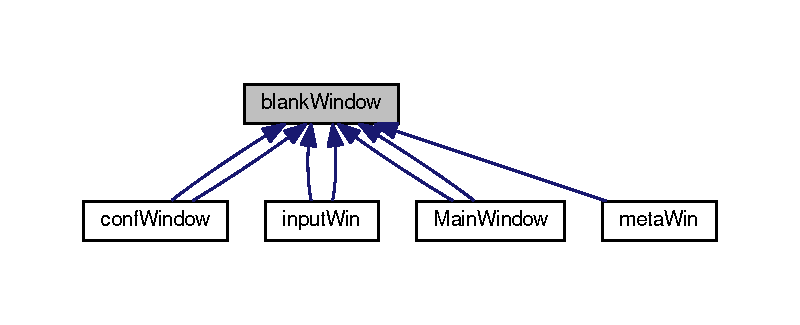
\includegraphics[width=350pt]{classgui_1_1window_1_1blankWindow__inherit__graph}
\end{center}
\end{figure}
\subsection*{Public Member Functions}
\begin{DoxyCompactItemize}
\item 
def \hyperlink{classgui_1_1window_1_1blankWindow_a2d865a6aea10146f28c546bed4ae1f44}{notdoneyet} (self)\hypertarget{classgui_1_1window_1_1blankWindow_a2d865a6aea10146f28c546bed4ae1f44}{}\label{classgui_1_1window_1_1blankWindow_a2d865a6aea10146f28c546bed4ae1f44}

\begin{DoxyCompactList}\small\item\em a simple dummy method for not yet implemented methods \end{DoxyCompactList}\end{DoxyCompactItemize}


\subsection{Detailed Description}
A simple window class with a not filled menu bar. 


\begin{DoxyParams}{Parameters}
{\em lang} & chosen language for the menu. \\
\hline
\end{DoxyParams}


The documentation for this class was generated from the following file\+:\begin{DoxyCompactItemize}
\item 
\hyperlink{window_8py}{window.\+py}\end{DoxyCompactItemize}

\hypertarget{classrpgtoolbox_1_1confbox_1_1chkCfg}{}\section{chk\+Cfg Class Reference}
\label{classrpgtoolbox_1_1confbox_1_1chkCfg}\index{chk\+Cfg@{chk\+Cfg}}


These Objects reads out a given config file and store the content of the configuration in a dictionary.  




Inherits object.

\subsection*{Public Member Functions}
\begin{DoxyCompactItemize}
\item 
def \hyperlink{classrpgtoolbox_1_1confbox_1_1chkCfg_a66e9d653925ded963afc456d24145c0a}{create\+Default} (self, path=\char`\"{}.\char`\"{}, filename=\char`\"{}default.\+conf\char`\"{}, logpath=\char`\"{}/tmp\char`\"{}, exp=\textquotesingle{}=\textquotesingle{}, comment=\textquotesingle{}\#\textquotesingle{})
\begin{DoxyCompactList}\small\item\em This method creates a default configuration file for the rpg-\/tools. \end{DoxyCompactList}\item 
def \hyperlink{classrpgtoolbox_1_1confbox_1_1chkCfg_a9757bd7448f940118f781e94d9c464c2}{save\+Cnf} (self, path=None, filename=\textquotesingle{}default.\+conf\textquotesingle{}, content=None)
\begin{DoxyCompactList}\small\item\em This method writes config data into a file. \end{DoxyCompactList}\end{DoxyCompactItemize}


\subsection{Detailed Description}
These Objects reads out a given config file and store the content of the configuration in a dictionary. 

\begin{DoxyRefDesc}{Todo}
\item[\hyperlink{todo__todo000013}{Todo}]read default config file if it exists in the same directory \end{DoxyRefDesc}


\subsection{Member Function Documentation}
\index{rpgtoolbox\+::confbox\+::chk\+Cfg@{rpgtoolbox\+::confbox\+::chk\+Cfg}!create\+Default@{create\+Default}}
\index{create\+Default@{create\+Default}!rpgtoolbox\+::confbox\+::chk\+Cfg@{rpgtoolbox\+::confbox\+::chk\+Cfg}}
\subsubsection[{\texorpdfstring{create\+Default(self, path=""."", filename=""default.\+conf"", logpath=""/tmp"", exp=\textquotesingle{}=\textquotesingle{}, comment=\textquotesingle{}\#\textquotesingle{})}{createDefault(self, path=".", filename="default.conf", logpath="/tmp", exp='=', comment='#')}}]{\setlength{\rightskip}{0pt plus 5cm}def create\+Default (
\begin{DoxyParamCaption}
\item[{}]{self, }
\item[{}]{path = {\ttfamily \char`\"{}.\char`\"{}}, }
\item[{}]{filename = {\ttfamily \char`\"{}default.conf\char`\"{}}, }
\item[{}]{logpath = {\ttfamily \char`\"{}/tmp\char`\"{}}, }
\item[{}]{exp = {\ttfamily \textquotesingle{}=\textquotesingle{}}, }
\item[{}]{comment = {\ttfamily \textquotesingle{}\#\textquotesingle{}}}
\end{DoxyParamCaption}
)}\hypertarget{classrpgtoolbox_1_1confbox_1_1chkCfg_a66e9d653925ded963afc456d24145c0a}{}\label{classrpgtoolbox_1_1confbox_1_1chkCfg_a66e9d653925ded963afc456d24145c0a}


This method creates a default configuration file for the rpg-\/tools. 


\begin{DoxyParams}{Parameters}
{\em path} & Path to the config file \\
\hline
{\em filname} & name of the config file \\
\hline
{\em exp} & expression for evaluate parameters \\
\hline
{\em comment} & comment character. \\
\hline
\end{DoxyParams}


Here is the call graph for this function\+:
\nopagebreak
\begin{figure}[H]
\begin{center}
\leavevmode
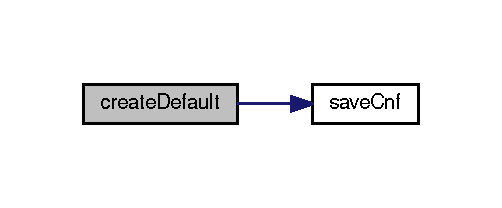
\includegraphics[width=241pt]{classrpgtoolbox_1_1confbox_1_1chkCfg_a66e9d653925ded963afc456d24145c0a_cgraph}
\end{center}
\end{figure}


\index{rpgtoolbox\+::confbox\+::chk\+Cfg@{rpgtoolbox\+::confbox\+::chk\+Cfg}!save\+Cnf@{save\+Cnf}}
\index{save\+Cnf@{save\+Cnf}!rpgtoolbox\+::confbox\+::chk\+Cfg@{rpgtoolbox\+::confbox\+::chk\+Cfg}}
\subsubsection[{\texorpdfstring{save\+Cnf(self, path=\+None, filename=\textquotesingle{}default.\+conf\textquotesingle{}, content=\+None)}{saveCnf(self, path=None, filename='default.conf', content=None)}}]{\setlength{\rightskip}{0pt plus 5cm}def save\+Cnf (
\begin{DoxyParamCaption}
\item[{}]{self, }
\item[{}]{path = {\ttfamily None}, }
\item[{}]{filename = {\ttfamily \textquotesingle{}default.conf\textquotesingle{}}, }
\item[{}]{content = {\ttfamily None}}
\end{DoxyParamCaption}
)}\hypertarget{classrpgtoolbox_1_1confbox_1_1chkCfg_a9757bd7448f940118f781e94d9c464c2}{}\label{classrpgtoolbox_1_1confbox_1_1chkCfg_a9757bd7448f940118f781e94d9c464c2}


This method writes config data into a file. 


\begin{DoxyParams}{Parameters}
{\em path} & path to the config file \\
\hline
{\em filename} & name of the config file \\
\hline
{\em content} & holds the content which shall be written to the config file. The used type for this should be a dictionary of the following structure\+: \{\textquotesingle{}config\+\_\+param\textquotesingle{} \+: value\} \\
\hline
\end{DoxyParams}


Here is the caller graph for this function\+:
\nopagebreak
\begin{figure}[H]
\begin{center}
\leavevmode
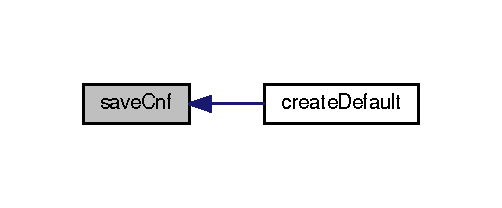
\includegraphics[width=241pt]{classrpgtoolbox_1_1confbox_1_1chkCfg_a9757bd7448f940118f781e94d9c464c2_icgraph}
\end{center}
\end{figure}




The documentation for this class was generated from the following file\+:\begin{DoxyCompactItemize}
\item 
\hyperlink{confbox_8py}{confbox.\+py}\end{DoxyCompactItemize}

\hypertarget{classgui_1_1window_1_1confWindow}{}\section{conf\+Window Class Reference}
\label{classgui_1_1window_1_1confWindow}\index{conf\+Window@{conf\+Window}}


This class builds a window for selecting and saving options of rpg-\/tools.  




Inheritance diagram for conf\+Window\+:
\nopagebreak
\begin{figure}[H]
\begin{center}
\leavevmode
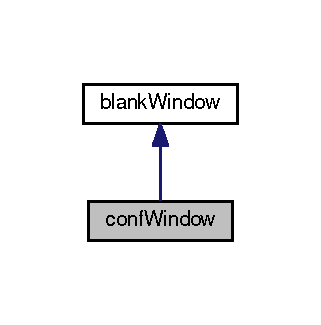
\includegraphics[width=154pt]{classgui_1_1window_1_1confWindow__inherit__graph}
\end{center}
\end{figure}


Collaboration diagram for conf\+Window\+:
\nopagebreak
\begin{figure}[H]
\begin{center}
\leavevmode
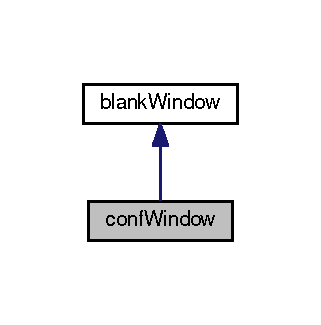
\includegraphics[width=154pt]{classgui_1_1window_1_1confWindow__coll__graph}
\end{center}
\end{figure}
\subsection*{Public Member Functions}
\begin{DoxyCompactItemize}
\item 
def \hyperlink{classgui_1_1window_1_1confWindow_a355ed316a41bdc8259ac11af5a2556f3}{chosen\+Lang} (self)\hypertarget{classgui_1_1window_1_1confWindow_a355ed316a41bdc8259ac11af5a2556f3}{}\label{classgui_1_1window_1_1confWindow_a355ed316a41bdc8259ac11af5a2556f3}

\begin{DoxyCompactList}\small\item\em A public method which return the string value of the chosen language. \end{DoxyCompactList}\end{DoxyCompactItemize}


\subsection{Detailed Description}
This class builds a window for selecting and saving options of rpg-\/tools. 

For now it is just choosing the language for menus and dialogues. 
\begin{DoxyParams}{Parameters}
{\em lang} & Laguage which shall be used in messages and menus. \\
\hline
\end{DoxyParams}


The documentation for this class was generated from the following file\+:\begin{DoxyCompactItemize}
\item 
\hyperlink{window_8py}{window.\+py}\end{DoxyCompactItemize}

\hypertarget{classcalc__ep_1_1confWindow}{}\section{conf\+Window Class Reference}
\label{classcalc__ep_1_1confWindow}\index{conf\+Window@{conf\+Window}}


This class builds a window for selecting and saving options of A\+Da\+ManT.  




Inheritance diagram for conf\+Window\+:
\nopagebreak
\begin{figure}[H]
\begin{center}
\leavevmode
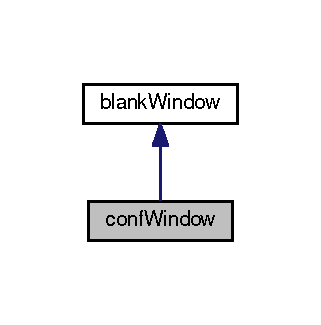
\includegraphics[width=154pt]{classcalc__ep_1_1confWindow__inherit__graph}
\end{center}
\end{figure}


Collaboration diagram for conf\+Window\+:
\nopagebreak
\begin{figure}[H]
\begin{center}
\leavevmode
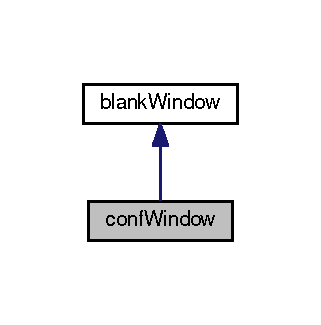
\includegraphics[width=154pt]{classcalc__ep_1_1confWindow__coll__graph}
\end{center}
\end{figure}
\subsection*{Public Member Functions}
\begin{DoxyCompactItemize}
\item 
def \hyperlink{classcalc__ep_1_1confWindow_a355ed316a41bdc8259ac11af5a2556f3}{chosen\+Lang} (self)\hypertarget{classcalc__ep_1_1confWindow_a355ed316a41bdc8259ac11af5a2556f3}{}\label{classcalc__ep_1_1confWindow_a355ed316a41bdc8259ac11af5a2556f3}

\begin{DoxyCompactList}\small\item\em A public method which return the string value of the chosen language. \end{DoxyCompactList}\end{DoxyCompactItemize}


\subsection{Detailed Description}
This class builds a window for selecting and saving options of A\+Da\+ManT. 

For now it is just choosing the language for menus and dialogues. 
\begin{DoxyParams}{Parameters}
{\em lang} & Laguage which shall be used in messages and menus. \\
\hline
\end{DoxyParams}


The documentation for this class was generated from the following file\+:\begin{DoxyCompactItemize}
\item 
\hyperlink{calc__ep_8py}{calc\+\_\+ep.\+py}\end{DoxyCompactItemize}

\hypertarget{classcalc__ep_1_1epSheet}{}\section{ep\+Sheet Class Reference}
\label{classcalc__ep_1_1epSheet}\index{ep\+Sheet@{ep\+Sheet}}


Class for calculating EP sheets.  




Inherits object.

\subsection*{Public Member Functions}
\begin{DoxyCompactItemize}
\item 
def \hyperlink{classcalc__ep_1_1epSheet_a2d865a6aea10146f28c546bed4ae1f44}{notdoneyet} (self)\hypertarget{classcalc__ep_1_1epSheet_a2d865a6aea10146f28c546bed4ae1f44}{}\label{classcalc__ep_1_1epSheet_a2d865a6aea10146f28c546bed4ae1f44}

\begin{DoxyCompactList}\small\item\em Most important dummy function. \end{DoxyCompactList}\end{DoxyCompactItemize}


\subsection{Detailed Description}
Class for calculating EP sheets. 

The documentation for this class was generated from the following file\+:\begin{DoxyCompactItemize}
\item 
\hyperlink{calc__ep_8py}{calc\+\_\+ep.\+py}\end{DoxyCompactItemize}

\hypertarget{classgui_1_1winhelper_1_1InfoCanvas}{}\section{Info\+Canvas Class Reference}
\label{classgui_1_1winhelper_1_1InfoCanvas}\index{Info\+Canvas@{Info\+Canvas}}


A Canvas-\/widget that holds a scrollable Message-\/widget.  




Inherits object.

\subsection*{Public Member Functions}
\begin{DoxyCompactItemize}
\item 
def \hyperlink{classgui_1_1winhelper_1_1InfoCanvas_a7a251b22287f6295a58ca328ef5bb9c0}{pack} (self, kw)\hypertarget{classgui_1_1winhelper_1_1InfoCanvas_a7a251b22287f6295a58ca328ef5bb9c0}{}\label{classgui_1_1winhelper_1_1InfoCanvas_a7a251b22287f6295a58ca328ef5bb9c0}

\begin{DoxyCompactList}\small\item\em Error handling method\+: This cannot be used with pack. \end{DoxyCompactList}\item 
def \hyperlink{classgui_1_1winhelper_1_1InfoCanvas_ab2a60e5dcddfee5a63307a872be5f05e}{place} (self, kw)\hypertarget{classgui_1_1winhelper_1_1InfoCanvas_ab2a60e5dcddfee5a63307a872be5f05e}{}\label{classgui_1_1winhelper_1_1InfoCanvas_ab2a60e5dcddfee5a63307a872be5f05e}

\begin{DoxyCompactList}\small\item\em Error handling method\+: This cannot be used with place. \end{DoxyCompactList}\end{DoxyCompactItemize}


\subsection{Detailed Description}
A Canvas-\/widget that holds a scrollable Message-\/widget. 

This widget can only be used by the grid() Geometry Manager.


\begin{DoxyParams}{Parameters}
{\em master} & master Tk()-\/object \\
\hline
{\em text} & text string that shall be displayed \\
\hline
{\em width} & width of the canvas in pixel \\
\hline
{\em row} & row index where to put this widget in the window structure \\
\hline
{\em column} & column index where to put this widget in the window structure \\
\hline
\end{DoxyParams}


The documentation for this class was generated from the following file\+:\begin{DoxyCompactItemize}
\item 
\hyperlink{winhelper_8py}{winhelper.\+py}\end{DoxyCompactItemize}

\hypertarget{classgui_1_1window_1_1inputWin}{}\section{input\+Win Class Reference}
\label{classgui_1_1window_1_1inputWin}\index{input\+Win@{input\+Win}}


Objects of this class type are windows for input the wanted data structure.  




Inheritance diagram for input\+Win\+:
\nopagebreak
\begin{figure}[H]
\begin{center}
\leavevmode
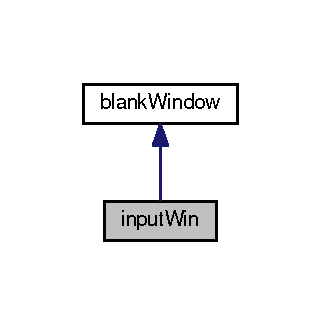
\includegraphics[width=154pt]{classgui_1_1window_1_1inputWin__inherit__graph}
\end{center}
\end{figure}


Collaboration diagram for input\+Win\+:
\nopagebreak
\begin{figure}[H]
\begin{center}
\leavevmode
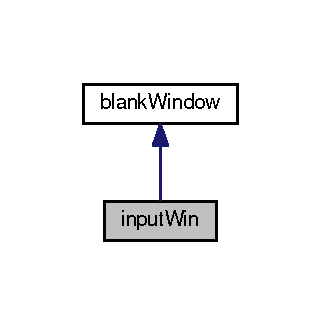
\includegraphics[width=154pt]{classgui_1_1window_1_1inputWin__coll__graph}
\end{center}
\end{figure}
\subsection*{Public Member Functions}
\begin{DoxyCompactItemize}
\item 
def \hyperlink{classgui_1_1window_1_1inputWin_a2d865a6aea10146f28c546bed4ae1f44}{notdoneyet} (self)\hypertarget{classgui_1_1window_1_1inputWin_a2d865a6aea10146f28c546bed4ae1f44}{}\label{classgui_1_1window_1_1inputWin_a2d865a6aea10146f28c546bed4ae1f44}

\begin{DoxyCompactList}\small\item\em Most important dummy method! \end{DoxyCompactList}\end{DoxyCompactItemize}


\subsection{Detailed Description}
Objects of this class type are windows for input the wanted data structure. 

A X\+ML structure will be build of the input. 
\begin{DoxyParams}{Parameters}
{\em lang} & This parameter holds the language chosen for the menus and messages. Default value is \textquotesingle{}en\textquotesingle{}. \\
\hline
{\em xmlcontent} & a dictionary holding the X\+ML structure/tags \\
\hline
{\em filename} & this holds the filename of a read X\+ML file holding the functional structure. \\
\hline
{\em storepath} & the path where the X\+ML files shall be stored in. \\
\hline
\end{DoxyParams}


The documentation for this class was generated from the following file\+:\begin{DoxyCompactItemize}
\item 
\hyperlink{window_8py}{window.\+py}\end{DoxyCompactItemize}

\hypertarget{classcalc__ep_1_1inputWin}{}\section{input\+Win Class Reference}
\label{classcalc__ep_1_1inputWin}\index{input\+Win@{input\+Win}}


Objects of this class type are windows for input the wanted data structure.  




Inheritance diagram for input\+Win\+:
\nopagebreak
\begin{figure}[H]
\begin{center}
\leavevmode
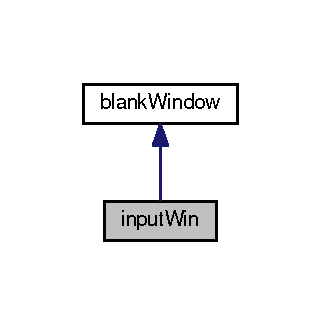
\includegraphics[width=154pt]{classcalc__ep_1_1inputWin__inherit__graph}
\end{center}
\end{figure}


Collaboration diagram for input\+Win\+:
\nopagebreak
\begin{figure}[H]
\begin{center}
\leavevmode
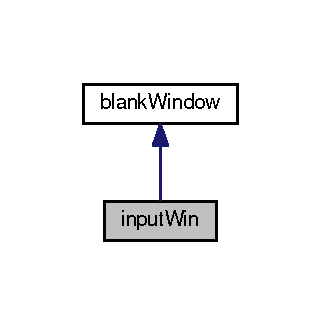
\includegraphics[width=154pt]{classcalc__ep_1_1inputWin__coll__graph}
\end{center}
\end{figure}
\subsection*{Public Member Functions}
\begin{DoxyCompactItemize}
\item 
def \hyperlink{classcalc__ep_1_1inputWin_a2d865a6aea10146f28c546bed4ae1f44}{notdoneyet} (self)\hypertarget{classcalc__ep_1_1inputWin_a2d865a6aea10146f28c546bed4ae1f44}{}\label{classcalc__ep_1_1inputWin_a2d865a6aea10146f28c546bed4ae1f44}

\begin{DoxyCompactList}\small\item\em Most important dummy method! \end{DoxyCompactList}\end{DoxyCompactItemize}


\subsection{Detailed Description}
Objects of this class type are windows for input the wanted data structure. 

A exp structure will be build of the input. 
\begin{DoxyParams}{Parameters}
{\em lang} & This parameter holds the language chosen for the menus and messages. Default value is \textquotesingle{}en\textquotesingle{}. \\
\hline
{\em filename} & this holds the filename of a read exp file holding the functional structure. \\
\hline
{\em storepath} & the path where the X\+ML files shall be stored in. \\
\hline
\end{DoxyParams}


The documentation for this class was generated from the following file\+:\begin{DoxyCompactItemize}
\item 
\hyperlink{calc__ep_8py}{calc\+\_\+ep.\+py}\end{DoxyCompactItemize}

\hypertarget{classrpgToolDefinitions_1_1MERSTables_1_1Magic}{}\section{Magic Class Reference}
\label{classrpgToolDefinitions_1_1MERSTables_1_1Magic}\index{Magic@{Magic}}


classdocs  




Inherits object.



\subsection{Detailed Description}
classdocs 

The documentation for this class was generated from the following file\+:\begin{DoxyCompactItemize}
\item 
\hyperlink{MERSTables_8py}{M\+E\+R\+S\+Tables.\+py}\end{DoxyCompactItemize}

\hypertarget{classgui_1_1window_1_1MainWindow}{}\section{Main\+Window Class Reference}
\label{classgui_1_1window_1_1MainWindow}\index{Main\+Window@{Main\+Window}}


This is the class for the main window object.  




Inheritance diagram for Main\+Window\+:
\nopagebreak
\begin{figure}[H]
\begin{center}
\leavevmode
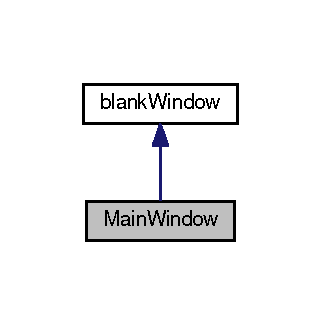
\includegraphics[width=154pt]{classgui_1_1window_1_1MainWindow__inherit__graph}
\end{center}
\end{figure}


Collaboration diagram for Main\+Window\+:
\nopagebreak
\begin{figure}[H]
\begin{center}
\leavevmode
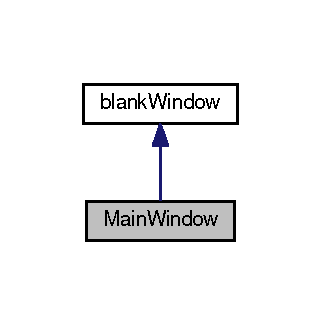
\includegraphics[width=154pt]{classgui_1_1window_1_1MainWindow__coll__graph}
\end{center}
\end{figure}
\subsection*{Public Member Functions}
\begin{DoxyCompactItemize}
\item 
def \hyperlink{classgui_1_1window_1_1MainWindow_a1ec143b7290b872531eb3198bf2fd45e}{help\+About} (self)\hypertarget{classgui_1_1window_1_1MainWindow_a1ec143b7290b872531eb3198bf2fd45e}{}\label{classgui_1_1window_1_1MainWindow_a1ec143b7290b872531eb3198bf2fd45e}

\begin{DoxyCompactList}\small\item\em This method just opens a message window with the basic information about the rpg-\/tools (like version and copyright) \end{DoxyCompactList}\item 
def \hyperlink{classgui_1_1window_1_1MainWindow_adf2bcf83729f963606d64edf1f739c03}{help\+Handbook} (self)
\begin{DoxyCompactList}\small\item\em This method will show the rpgbox Handbook. \end{DoxyCompactList}\item 
def \hyperlink{classgui_1_1window_1_1MainWindow_a2d865a6aea10146f28c546bed4ae1f44}{notdoneyet} (self)\hypertarget{classgui_1_1window_1_1MainWindow_a2d865a6aea10146f28c546bed4ae1f44}{}\label{classgui_1_1window_1_1MainWindow_a2d865a6aea10146f28c546bed4ae1f44}

\begin{DoxyCompactList}\small\item\em An I\+M\+P\+O\+R\+T\+A\+NT dummy for methods which are not implemented yet ;-\/) \end{DoxyCompactList}\item 
def \hyperlink{classgui_1_1window_1_1MainWindow_adc2ac7ec0038032ab9047f57fa52ba32}{opt\+Win} (self)\hypertarget{classgui_1_1window_1_1MainWindow_adc2ac7ec0038032ab9047f57fa52ba32}{}\label{classgui_1_1window_1_1MainWindow_adc2ac7ec0038032ab9047f57fa52ba32}

\begin{DoxyCompactList}\small\item\em Opens an option window and closes the main window. \end{DoxyCompactList}\end{DoxyCompactItemize}


\subsection{Detailed Description}
This is the class for the main window object. 


\begin{DoxyParams}{Parameters}
{\em lang} & The chosen language for window\textquotesingle{}s and button\textquotesingle{}s texts. At the moment, only English (en, default value) and German (de) are supported. \\
\hline
\end{DoxyParams}


\subsection{Member Function Documentation}
\index{gui\+::window\+::\+Main\+Window@{gui\+::window\+::\+Main\+Window}!help\+Handbook@{help\+Handbook}}
\index{help\+Handbook@{help\+Handbook}!gui\+::window\+::\+Main\+Window@{gui\+::window\+::\+Main\+Window}}
\subsubsection[{\texorpdfstring{help\+Handbook(self)}{helpHandbook(self)}}]{\setlength{\rightskip}{0pt plus 5cm}def help\+Handbook (
\begin{DoxyParamCaption}
\item[{}]{self}
\end{DoxyParamCaption}
)}\hypertarget{classgui_1_1window_1_1MainWindow_adf2bcf83729f963606d64edf1f739c03}{}\label{classgui_1_1window_1_1MainWindow_adf2bcf83729f963606d64edf1f739c03}


This method will show the rpgbox Handbook. 

\begin{DoxyRefDesc}{Todo}
\item[\hyperlink{todo__todo000009}{Todo}]help\+Handbook needs to be implemented \end{DoxyRefDesc}


Here is the call graph for this function\+:
\nopagebreak
\begin{figure}[H]
\begin{center}
\leavevmode
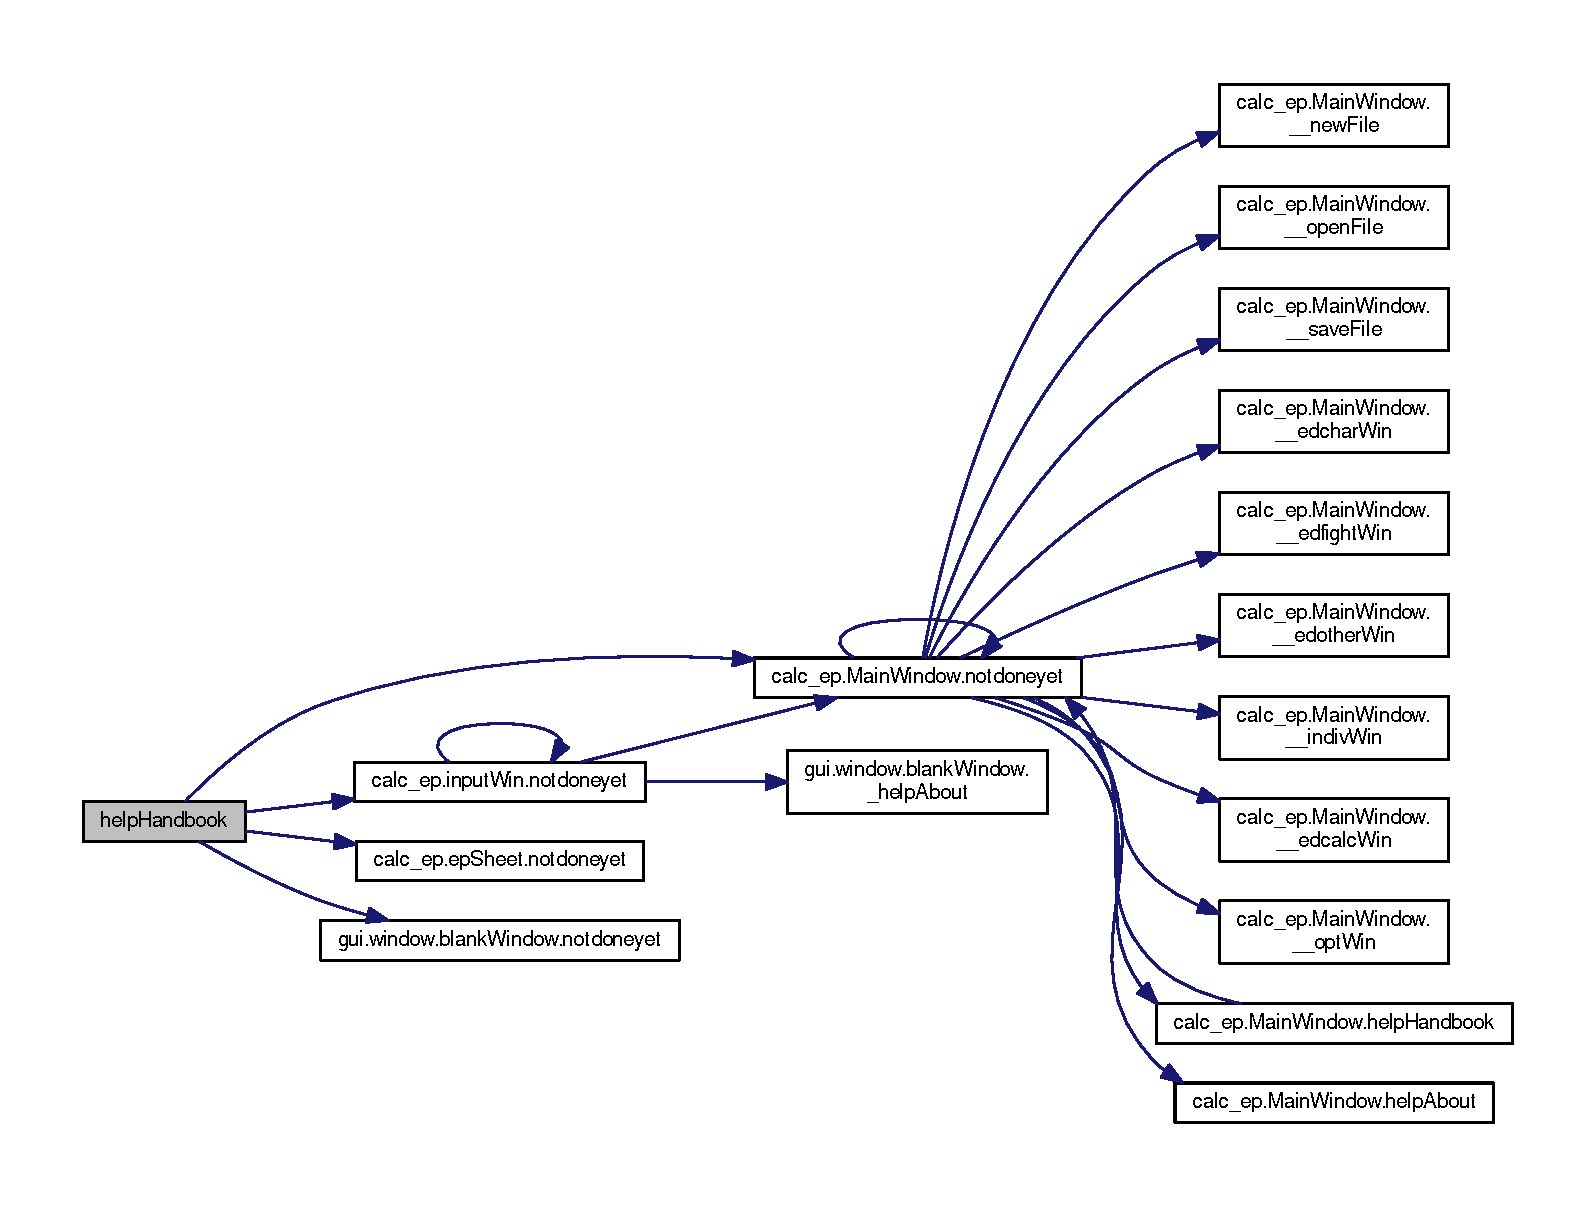
\includegraphics[width=350pt]{classgui_1_1window_1_1MainWindow_adf2bcf83729f963606d64edf1f739c03_cgraph}
\end{center}
\end{figure}




Here is the caller graph for this function\+:
\nopagebreak
\begin{figure}[H]
\begin{center}
\leavevmode
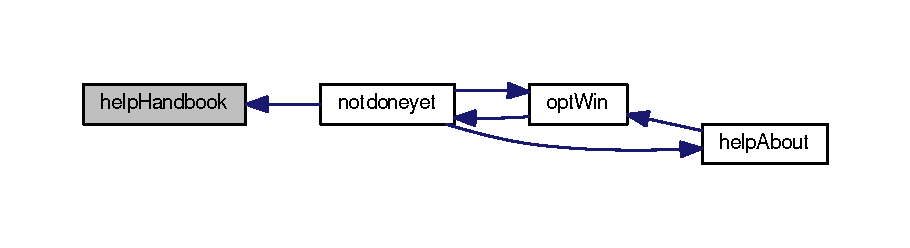
\includegraphics[width=350pt]{classgui_1_1window_1_1MainWindow_adf2bcf83729f963606d64edf1f739c03_icgraph}
\end{center}
\end{figure}




The documentation for this class was generated from the following file\+:\begin{DoxyCompactItemize}
\item 
\hyperlink{window_8py}{window.\+py}\end{DoxyCompactItemize}

\hypertarget{classcalc__ep_1_1MainWindow}{}\section{Main\+Window Class Reference}
\label{classcalc__ep_1_1MainWindow}\index{Main\+Window@{Main\+Window}}


This is the class for the main window object.  




Inheritance diagram for Main\+Window\+:
\nopagebreak
\begin{figure}[H]
\begin{center}
\leavevmode
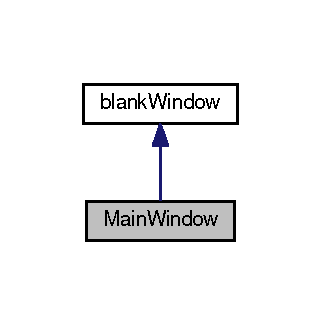
\includegraphics[width=154pt]{classcalc__ep_1_1MainWindow__inherit__graph}
\end{center}
\end{figure}


Collaboration diagram for Main\+Window\+:
\nopagebreak
\begin{figure}[H]
\begin{center}
\leavevmode
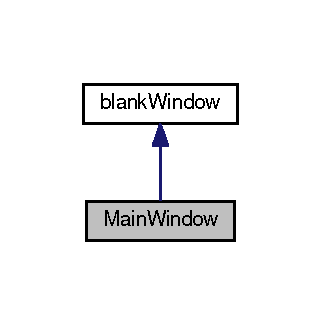
\includegraphics[width=154pt]{classcalc__ep_1_1MainWindow__coll__graph}
\end{center}
\end{figure}
\subsection*{Public Member Functions}
\begin{DoxyCompactItemize}
\item 
def \hyperlink{classcalc__ep_1_1MainWindow_a1ec143b7290b872531eb3198bf2fd45e}{help\+About} (self)\hypertarget{classcalc__ep_1_1MainWindow_a1ec143b7290b872531eb3198bf2fd45e}{}\label{classcalc__ep_1_1MainWindow_a1ec143b7290b872531eb3198bf2fd45e}

\begin{DoxyCompactList}\small\item\em This method just opens a message window with the basic information about the P\+R\+O\+G\+R\+AM (like version and copyright) \end{DoxyCompactList}\item 
def \hyperlink{classcalc__ep_1_1MainWindow_adf2bcf83729f963606d64edf1f739c03}{help\+Handbook} (self)
\begin{DoxyCompactList}\small\item\em This method will show the A\+Da\+ManT Handbook. \end{DoxyCompactList}\item 
def \hyperlink{classcalc__ep_1_1MainWindow_a2d865a6aea10146f28c546bed4ae1f44}{notdoneyet} (self)\hypertarget{classcalc__ep_1_1MainWindow_a2d865a6aea10146f28c546bed4ae1f44}{}\label{classcalc__ep_1_1MainWindow_a2d865a6aea10146f28c546bed4ae1f44}

\begin{DoxyCompactList}\small\item\em An I\+M\+P\+O\+R\+T\+A\+NT dummy for methods which are not implemented yet ;-\/) \end{DoxyCompactList}\end{DoxyCompactItemize}


\subsection{Detailed Description}
This is the class for the main window object. 


\begin{DoxyParams}{Parameters}
{\em lang} & The chosen language for window\textquotesingle{}s and button\textquotesingle{}s texts. At the moment, only English (en, default value) and German (de) are supported. \\
\hline
{\em title} & title of the window \\
\hline
{\em storepath} & path where things like options have to be stored \\
\hline
\end{DoxyParams}


\subsection{Member Function Documentation}
\index{calc\+\_\+ep\+::\+Main\+Window@{calc\+\_\+ep\+::\+Main\+Window}!help\+Handbook@{help\+Handbook}}
\index{help\+Handbook@{help\+Handbook}!calc\+\_\+ep\+::\+Main\+Window@{calc\+\_\+ep\+::\+Main\+Window}}
\subsubsection[{\texorpdfstring{help\+Handbook(self)}{helpHandbook(self)}}]{\setlength{\rightskip}{0pt plus 5cm}def help\+Handbook (
\begin{DoxyParamCaption}
\item[{}]{self}
\end{DoxyParamCaption}
)}\hypertarget{classcalc__ep_1_1MainWindow_adf2bcf83729f963606d64edf1f739c03}{}\label{classcalc__ep_1_1MainWindow_adf2bcf83729f963606d64edf1f739c03}


This method will show the A\+Da\+ManT Handbook. 

\begin{DoxyRefDesc}{Todo}
\item[\hyperlink{todo__todo000004}{Todo}]this needs to be implemented \end{DoxyRefDesc}


Here is the call graph for this function\+:
\nopagebreak
\begin{figure}[H]
\begin{center}
\leavevmode
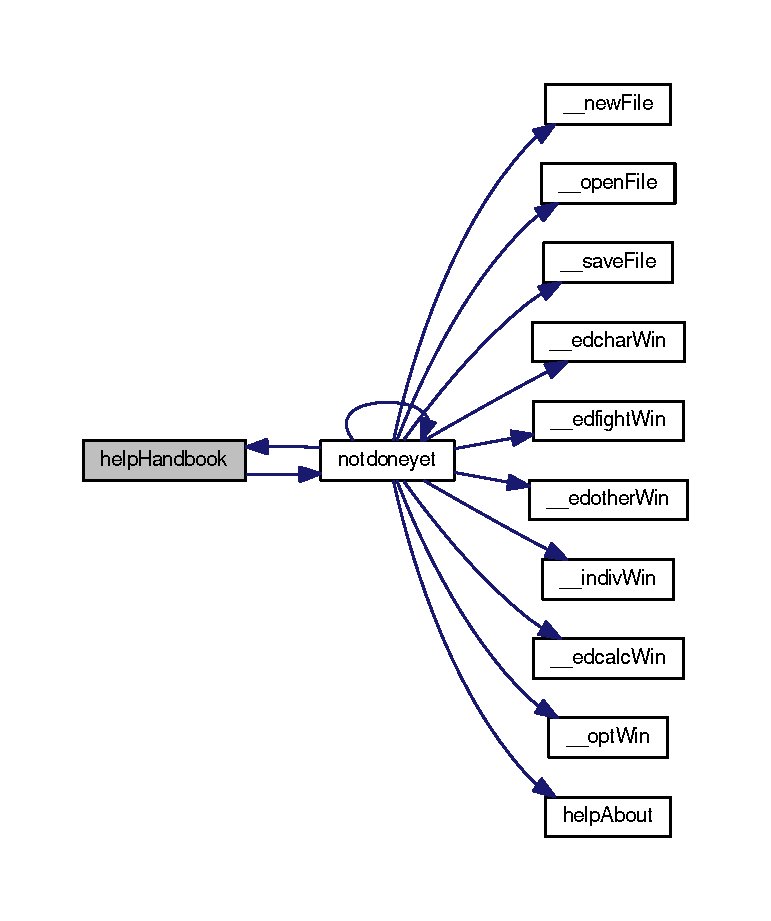
\includegraphics[width=350pt]{classcalc__ep_1_1MainWindow_adf2bcf83729f963606d64edf1f739c03_cgraph}
\end{center}
\end{figure}




Here is the caller graph for this function\+:
\nopagebreak
\begin{figure}[H]
\begin{center}
\leavevmode
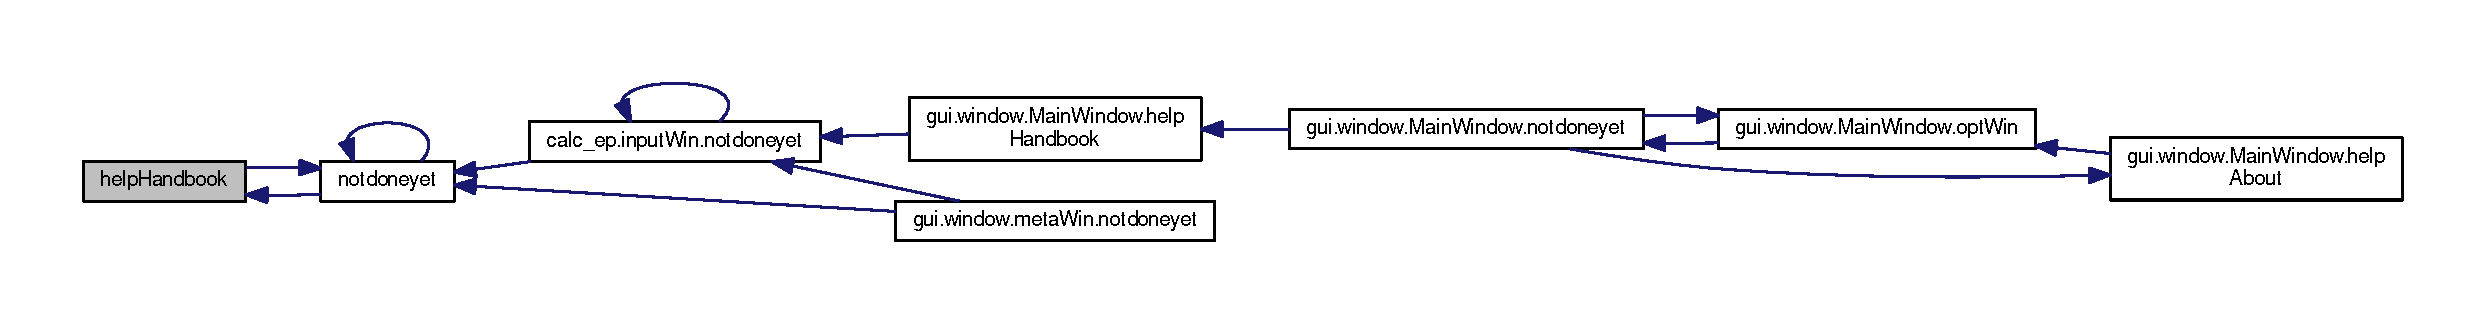
\includegraphics[width=350pt]{classcalc__ep_1_1MainWindow_adf2bcf83729f963606d64edf1f739c03_icgraph}
\end{center}
\end{figure}




The documentation for this class was generated from the following file\+:\begin{DoxyCompactItemize}
\item 
\hyperlink{calc__ep_8py}{calc\+\_\+ep.\+py}\end{DoxyCompactItemize}

\hypertarget{classgui_1_1window_1_1messageWindow}{}\section{message\+Window Class Reference}
\label{classgui_1_1window_1_1messageWindow}\index{message\+Window@{message\+Window}}


A class to build a message window containing version, author and email on default.  




Inherits object.

\subsection*{Public Member Functions}
\begin{DoxyCompactItemize}
\item 
def \hyperlink{classgui_1_1window_1_1messageWindow_ac363d9b210b00523bd2d7b73e5f1a2dd}{showinfo} (self, message=\textquotesingle{}\textquotesingle{}, title=\textquotesingle{}Info\textquotesingle{})
\begin{DoxyCompactList}\small\item\em This method adds and displays content to the message window. \end{DoxyCompactList}\end{DoxyCompactItemize}


\subsection{Detailed Description}
A class to build a message window containing version, author and email on default. 


\begin{DoxyParams}{Parameters}
{\em lang} & contains the chosen display language. \\
\hline
\end{DoxyParams}


\subsection{Member Function Documentation}
\index{gui\+::window\+::message\+Window@{gui\+::window\+::message\+Window}!showinfo@{showinfo}}
\index{showinfo@{showinfo}!gui\+::window\+::message\+Window@{gui\+::window\+::message\+Window}}
\subsubsection[{\texorpdfstring{showinfo(self, message=\textquotesingle{}\textquotesingle{}, title=\textquotesingle{}\+Info\textquotesingle{})}{showinfo(self, message='', title='Info')}}]{\setlength{\rightskip}{0pt plus 5cm}def showinfo (
\begin{DoxyParamCaption}
\item[{}]{self, }
\item[{}]{message = {\ttfamily \textquotesingle{}\textquotesingle{}}, }
\item[{}]{title = {\ttfamily \textquotesingle{}Info\textquotesingle{}}}
\end{DoxyParamCaption}
)}\hypertarget{classgui_1_1window_1_1messageWindow_ac363d9b210b00523bd2d7b73e5f1a2dd}{}\label{classgui_1_1window_1_1messageWindow_ac363d9b210b00523bd2d7b73e5f1a2dd}


This method adds and displays content to the message window. 


\begin{DoxyParams}{Parameters}
{\em message} & contains a message to be displayed in the message window. It may be an array, a string or a number (integer/float). \\
\hline
{\em title} & sets the title of the message window. The default is \textquotesingle{}Info\textquotesingle{}. \\
\hline
\end{DoxyParams}


The documentation for this class was generated from the following file\+:\begin{DoxyCompactItemize}
\item 
\hyperlink{window_8py}{window.\+py}\end{DoxyCompactItemize}

\hypertarget{classgui_1_1window_1_1metaWin}{}\section{meta\+Win Class Reference}
\label{classgui_1_1window_1_1metaWin}\index{meta\+Win@{meta\+Win}}


Creates a window for generating meta data fields.  




Inheritance diagram for meta\+Win\+:
\nopagebreak
\begin{figure}[H]
\begin{center}
\leavevmode
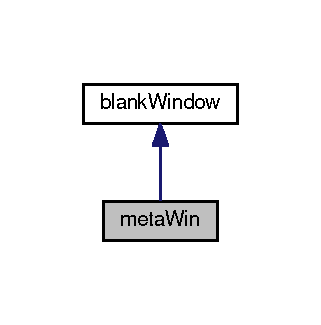
\includegraphics[width=154pt]{classgui_1_1window_1_1metaWin__inherit__graph}
\end{center}
\end{figure}


Collaboration diagram for meta\+Win\+:
\nopagebreak
\begin{figure}[H]
\begin{center}
\leavevmode
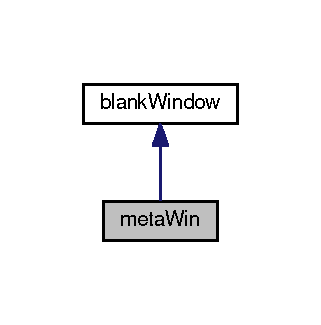
\includegraphics[width=154pt]{classgui_1_1window_1_1metaWin__coll__graph}
\end{center}
\end{figure}
\subsection*{Public Member Functions}
\begin{DoxyCompactItemize}
\item 
def \hyperlink{classgui_1_1window_1_1metaWin_a2d865a6aea10146f28c546bed4ae1f44}{notdoneyet} (self)\hypertarget{classgui_1_1window_1_1metaWin_a2d865a6aea10146f28c546bed4ae1f44}{}\label{classgui_1_1window_1_1metaWin_a2d865a6aea10146f28c546bed4ae1f44}

\begin{DoxyCompactList}\small\item\em Most important dummy method! \end{DoxyCompactList}\end{DoxyCompactItemize}


\subsection{Detailed Description}
Creates a window for generating meta data fields. 


\begin{DoxyParams}{Parameters}
{\em lang} & this holds the chosen display language. \\
\hline
{\em storepath} & path of the default storage location of the X\+ML files. \\
\hline
\end{DoxyParams}


The documentation for this class was generated from the following file\+:\begin{DoxyCompactItemize}
\item 
\hyperlink{window_8py}{window.\+py}\end{DoxyCompactItemize}

\hypertarget{classrpgToolDefinitions_1_1RMTables_1_1MyClass}{}\section{My\+Class Class Reference}
\label{classrpgToolDefinitions_1_1RMTables_1_1MyClass}\index{My\+Class@{My\+Class}}


Created on 13.\+12.\+2015.  




Inherits object.



\subsection{Detailed Description}
Created on 13.\+12.\+2015. 

\begin{DoxyAuthor}{Author}
\+: mongol \begin{DoxyVerb}classdocs\end{DoxyVerb}
 
\end{DoxyAuthor}


The documentation for this class was generated from the following file\+:\begin{DoxyCompactItemize}
\item 
R\+M\+Tables.\+py\end{DoxyCompactItemize}

\hypertarget{classrpgtoolbox_1_1errbox_1_1raisedError}{}\section{raised\+Error Class Reference}
\label{classrpgtoolbox_1_1errbox_1_1raisedError}\index{raised\+Error@{raised\+Error}}


Objects of this class will be raised in case of errors with files used for rpg-\/tools.  




Inherits Exception.



\subsection{Detailed Description}
Objects of this class will be raised in case of errors with files used for rpg-\/tools. 


\begin{DoxyParams}{Parameters}
{\em value} & the value to be given to the error handler (e.\+g., message) \\
\hline
\end{DoxyParams}


The documentation for this class was generated from the following file\+:\begin{DoxyCompactItemize}
\item 
\hyperlink{errbox_8py}{errbox.\+py}\end{DoxyCompactItemize}

\chapter{File Documentation}
\hypertarget{Backpack_8py}{}\section{Backpack.\+py File Reference}
\label{Backpack_8py}\index{Backpack.\+py@{Backpack.\+py}}


This is a simple tool to keep track of a character\textquotesingle{}s backpack.  




\subsection{Detailed Description}
This is a simple tool to keep track of a character\textquotesingle{}s backpack. 

With this tool you are able to keep track of all the items and the money a pen \& paper R\+PG character is carrying. To make it work as an \char`\"{}\+Online Shop\char`\"{} you need to set up a My\+S\+QL data base.

\begin{DoxyDate}{Date}
(C) 2015 
\end{DoxyDate}
\begin{DoxyAuthor}{Author}
Marcus Schwamberger  \href{mailto:marcus@lederzeug.de}{\tt marcus@lederzeug.\+de}
\end{DoxyAuthor}
\begin{DoxyRefDesc}{Todo}
\item[\hyperlink{todo__todo000001}{Todo}]Modul\+: reading and interpreting mysql configuration 

Modul\+: create intial mysql db 

Modul\+: insert, update and read data from db 

Modul\+: saves extracted data as P\+DF \end{DoxyRefDesc}

\hypertarget{calc__ep_8py}{}\section{calc\+\_\+ep.\+py File Reference}
\label{calc__ep_8py}\index{calc\+\_\+ep.\+py@{calc\+\_\+ep.\+py}}
\subsection*{Data Structures}
\begin{DoxyCompactItemize}
\item 
class \hyperlink{classcalc__ep_1_1confWindow}{conf\+Window}
\begin{DoxyCompactList}\small\item\em This class builds a window for selecting and saving options of A\+Da\+ManT. \end{DoxyCompactList}\item 
class \hyperlink{classcalc__ep_1_1epSheet}{ep\+Sheet}
\begin{DoxyCompactList}\small\item\em Class for calculating EP sheets. \end{DoxyCompactList}\item 
class \hyperlink{classcalc__ep_1_1inputWin}{input\+Win}
\begin{DoxyCompactList}\small\item\em Objects of this class type are windows for input the wanted data structure. \end{DoxyCompactList}\item 
class \hyperlink{classcalc__ep_1_1MainWindow}{Main\+Window}
\begin{DoxyCompactList}\small\item\em This is the class for the main window object. \end{DoxyCompactList}\end{DoxyCompactItemize}
\subsection*{Namespaces}
\begin{DoxyCompactItemize}
\item 
 \hyperlink{namespacecalc__ep}{calc\+\_\+ep}
\begin{DoxyCompactList}\small\item\em This is a little tool for calculating E\+Ps for M\+E\+R\+S/\+RM. \end{DoxyCompactList}\end{DoxyCompactItemize}

\hypertarget{confbox_8py}{}\section{confbox.\+py File Reference}
\label{confbox_8py}\index{confbox.\+py@{confbox.\+py}}


A toolbox of things to handle config files.  


\subsection*{Data Structures}
\begin{DoxyCompactItemize}
\item 
class \hyperlink{classrpgtoolbox_1_1confbox_1_1chkCfg}{chk\+Cfg}
\begin{DoxyCompactList}\small\item\em These Objects reads out a given config file and store the content of the configuration in a dictionary. \end{DoxyCompactList}\end{DoxyCompactItemize}
\subsection*{Variables}
\begin{DoxyCompactItemize}
\item 
dictionary \hyperlink{confbox_8py_a7ed6b9a6c432c881b9733171f0b70cd8}{cfgopts}\hypertarget{confbox_8py_a7ed6b9a6c432c881b9733171f0b70cd8}{}\label{confbox_8py_a7ed6b9a6c432c881b9733171f0b70cd8}

\begin{DoxyCompactList}\small\item\em cfgopts holds allowed configuration options and their descriptions \end{DoxyCompactList}\item 
dictionary \hyperlink{confbox_8py_afcd7470d4ff2621f87d41d72656e4672}{defval}
\begin{DoxyCompactList}\small\item\em defval holds default values for a configuration file. \end{DoxyCompactList}\item 
\hyperlink{confbox_8py_ae20c0a4ad8d34be878098ec1a1998ff9}{home} = os.\+path.\+expanduser(\textquotesingle{}$\sim$\textquotesingle{})\hypertarget{confbox_8py_ae20c0a4ad8d34be878098ec1a1998ff9}{}\label{confbox_8py_ae20c0a4ad8d34be878098ec1a1998ff9}

\begin{DoxyCompactList}\small\item\em home holds users home directory \end{DoxyCompactList}\end{DoxyCompactItemize}


\subsection{Detailed Description}
A toolbox of things to handle config files. 

\begin{DoxyAuthor}{Author}
Marcus Schwamberger 
\end{DoxyAuthor}
\begin{DoxyDate}{Date}
(c) 2012-\/2016 
\end{DoxyDate}
\begin{DoxyVersion}{Version}
0.\+5.\+2 alpha  \href{mailto:marcus@lederzeug.de}{\tt marcus@lederzeug.\+de}  G\+NU V3.\+0 
\end{DoxyVersion}


\subsection{Variable Documentation}
\index{confbox.\+py@{confbox.\+py}!defval@{defval}}
\index{defval@{defval}!confbox.\+py@{confbox.\+py}}
\subsubsection[{\texorpdfstring{defval}{defval}}]{\setlength{\rightskip}{0pt plus 5cm}dictionary defval}\hypertarget{confbox_8py_file_afcd7470d4ff2621f87d41d72656e4672}{}\label{confbox_8py_file_afcd7470d4ff2621f87d41d72656e4672}
{\bfseries Initial value\+:}
\begin{DoxyCode}
1 = \{\textcolor{stringliteral}{'lang'} : \textcolor{stringliteral}{'en'},
2           \textcolor{stringliteral}{'datapath'} : \textcolor{stringliteral}{'./data'},
3           \textcolor{stringliteral}{'logpath'}  : \textcolor{stringliteral}{'/tmp/'},
4           \textcolor{stringliteral}{'logcount'} : 5,
5           \textcolor{stringliteral}{'logsize'}  : \textcolor{stringliteral}{'1M'},
6           \textcolor{stringliteral}{'logfile'}  : \textcolor{stringliteral}{'rpgtools.log'},
7           \textcolor{stringliteral}{'loglevel'} : \textcolor{stringliteral}{'error'},
8           \textcolor{stringliteral}{'db\_type'}  : \textcolor{stringliteral}{'csv'},
9           \textcolor{stringliteral}{'db\_host'}  : \textcolor{stringliteral}{'localhost'},
10           \textcolor{stringliteral}{'db\_port'}  : 3306,
11           \textcolor{stringliteral}{'db\_user'}  : \textcolor{stringliteral}{'rpgtools'},
12           \textcolor{stringliteral}{'db\_passwd'}: \textcolor{stringliteral}{'secred'},
13           \textcolor{stringliteral}{'calc\_type'}: \textcolor{stringliteral}{'simple'},
14           
15           \}
\end{DoxyCode}


defval holds default values for a configuration file. 


\hypertarget{epcalcdefs_8py}{}\section{epcalcdefs.\+py File Reference}
\label{epcalcdefs_8py}\index{epcalcdefs.\+py@{epcalcdefs.\+py}}
\subsection*{Namespaces}
\begin{DoxyCompactItemize}
\item 
 \hyperlink{namespacerpgToolDefinitions_1_1epcalcdefs}{rpg\+Tool\+Definitions.\+epcalcdefs}
\begin{DoxyCompactList}\small\item\em Definitions for E\+P-\/\+Calculator This module contains predefined variables, lists, etc. \end{DoxyCompactList}\end{DoxyCompactItemize}
\subsection*{Functions}
\begin{DoxyCompactItemize}
\item 
def \hyperlink{namespacerpgToolDefinitions_1_1epcalcdefs_a0c04e5f498010d3ae4df2afba7b414c8}{calc\+E\+P\+Spell} (spell=1, caster=1)
\begin{DoxyCompactList}\small\item\em This function returns the EP for a cast spell. \end{DoxyCompactList}\item 
def \hyperlink{namespacerpgToolDefinitions_1_1epcalcdefs_abf04e7e0e98cc6f560af932d5117f716}{get\+E\+P\+Crit} (level=0, crit=\char`\"{}A\char`\"{}, charhit=False)
\begin{DoxyCompactList}\small\item\em This function returns the EP for a gained or provoked critical hit. \end{DoxyCompactList}\end{DoxyCompactItemize}

\hypertarget{errbox_8py}{}\section{errbox.\+py File Reference}
\label{errbox_8py}\index{errbox.\+py@{errbox.\+py}}


A box full of error classes.  


\subsection*{Data Structures}
\begin{DoxyCompactItemize}
\item 
class \hyperlink{classrpgtoolbox_1_1errbox_1_1raisedError}{raised\+Error}
\begin{DoxyCompactList}\small\item\em Objects of this class will be raised in case of errors with files used for rpg-\/tools. \end{DoxyCompactList}\end{DoxyCompactItemize}


\subsection{Detailed Description}
A box full of error classes. 

\begin{DoxyDate}{Date}
(C) 2012-\/2016 
\end{DoxyDate}
\begin{DoxyAuthor}{Author}
Marcus Schwamberger  \href{mailto:marcus@lederzeug.de}{\tt marcus@lederzeug.\+de} 
\end{DoxyAuthor}
\begin{DoxyVersion}{Version}
0.\+1 alpha 
\end{DoxyVersion}

\hypertarget{globaltools_8py}{}\section{globaltools.\+py File Reference}
\label{globaltools_8py}\index{globaltools.\+py@{globaltools.\+py}}


a bunch of nice global tools.  


\subsection*{Functions}
\begin{DoxyCompactItemize}
\item 
def \hyperlink{globaltools_8py_a7837b18e219c540d8a30bd9631314a0a}{array2dict} (array=\mbox{[}$\,$\mbox{]}, expr=\textquotesingle{}=\textquotesingle{}, comment=\textquotesingle{}\#\textquotesingle{})
\begin{DoxyCompactList}\small\item\em This function transforms an array $<$str1$>$=$<$str2$>$ into a dictionary \{ $<$str1$>$ \+: $<$str2$>$\}. \end{DoxyCompactList}\item 
def \hyperlink{globaltools_8py_a169a201fcc606a30afa380587cbc6c09}{asci\+Loops} (way=\mbox{[}$\,$\mbox{]}, element=\char`\"{}\char`\"{})
\begin{DoxyCompactList}\small\item\em This is a small helper function to display a loop from a list as \textquotesingle{}asci\textquotesingle{}. \end{DoxyCompactList}\item 
def \hyperlink{globaltools_8py_a80518a0197675bea51148d1c3cd40279}{check\+Exist} (arg=\char`\"{}\char`\"{})
\begin{DoxyCompactList}\small\item\em This function checks whether given argument (object/variable/list...) already exists or not. \end{DoxyCompactList}\item 
def \hyperlink{globaltools_8py_ab12184b6cf7857bd9d51fc9af4ab1f52}{check\+Files} (path=\textquotesingle{}./\textquotesingle{}, file\+\_\+list=\mbox{[}$\,$\mbox{]})
\begin{DoxyCompactList}\small\item\em This function check out whether a list of files exists in a specific directory. \end{DoxyCompactList}\item 
def \hyperlink{globaltools_8py_a87c99a26e79147d5025cfdfda26dc57d}{count\+Elem} (elem=\textquotesingle{}\textquotesingle{}, alist=\mbox{[}$\,$\mbox{]})
\begin{DoxyCompactList}\small\item\em This tiny functions just count the occurrences of an element in a list. \end{DoxyCompactList}\item 
def \hyperlink{globaltools_8py_a388d233340dff99be67f0afc03953992}{find\+Loops} (struc=\{\}, elem=\textquotesingle{}\textquotesingle{}, way=\mbox{[}$\,$\mbox{]}, result=\mbox{[}$\,$\mbox{]})
\begin{DoxyCompactList}\small\item\em This function looks for loops in a tree structure. \end{DoxyCompactList}\item 
def \hyperlink{globaltools_8py_a26eac5d473aed10e2965d37099bf9e5e}{get\+Last} (string=\char`\"{}/\char`\"{}, sep=\textquotesingle{}/\textquotesingle{})
\begin{DoxyCompactList}\small\item\em This function gives the last element of a list stored in a string. \end{DoxyCompactList}\item 
def \hyperlink{globaltools_8py_a748b3ad515bb5f8281892b7f82a7ff4b}{list2str} (array=\mbox{[}$\,$\mbox{]})
\begin{DoxyCompactList}\small\item\em This function transforms a list/tuple into a string where the elements are separated by spaces. \end{DoxyCompactList}\item 
def \hyperlink{globaltools_8py_a4eea1f0cbce0bb32cd15f2f6847a40b5}{make\+Key\+List} (dic=\{\}, klist=\mbox{[}$\,$\mbox{]})
\begin{DoxyCompactList}\small\item\em This function simply extracts/compares the key index of a given dictionary with a list. \end{DoxyCompactList}\item 
def \hyperlink{globaltools_8py_a3f1400c5d3ed1fc184f85581b8aedc1a}{read\+File} (path=\textquotesingle{}./\textquotesingle{}, file\+\_\+name=None, mode=\textquotesingle{}r\textquotesingle{})
\begin{DoxyCompactList}\small\item\em This function reads a file and returns its content. \end{DoxyCompactList}\item 
def \hyperlink{globaltools_8py_a65b43889cc476f29c33c6e9f22b368a7}{sort\+Index} (dic=\{\})
\begin{DoxyCompactList}\small\item\em This function is a little helper when sorting a dictionary. \end{DoxyCompactList}\item 
def \hyperlink{globaltools_8py_a5b344d6078286fff96c81ccfdb524aa6}{tstr2list} (string=\textquotesingle{}(1, 2, 3)\textquotesingle{})
\begin{DoxyCompactList}\small\item\em This function transforms a string which \textquotesingle{}looks like a tuple\textquotesingle{} into a list. \end{DoxyCompactList}\item 
def \hyperlink{globaltools_8py_ad297bc6fb6b7b3a45a467248ce2ba004}{write\+File} (path=\textquotesingle{}./\textquotesingle{}, file\+\_\+name=\textquotesingle{}output\textquotesingle{}, data=None, mode=\textquotesingle{}w\textquotesingle{})
\begin{DoxyCompactList}\small\item\em This function simply (over)writes a file with given data. \end{DoxyCompactList}\end{DoxyCompactItemize}


\subsection{Detailed Description}
a bunch of nice global tools. 

This module holds some nice small helper functions like I/O things.

\begin{DoxyAuthor}{Author}
Marcus Schwamberger 
\end{DoxyAuthor}
\begin{DoxyDate}{Date}
(c) 2012-\/2016 
\end{DoxyDate}
\begin{DoxyVersion}{Version}
0.\+5.\+4 alpha  \href{mailto:marcus@lederzeug.de}{\tt marcus@lederzeug.\+de} 
\end{DoxyVersion}


\subsection{Function Documentation}
\index{globaltools.\+py@{globaltools.\+py}!array2dict@{array2dict}}
\index{array2dict@{array2dict}!globaltools.\+py@{globaltools.\+py}}
\subsubsection[{\texorpdfstring{array2dict(array=[], expr=\textquotesingle{}=\textquotesingle{}, comment=\textquotesingle{}\#\textquotesingle{})}{array2dict(array=[], expr='=', comment='#')}}]{\setlength{\rightskip}{0pt plus 5cm}def rpgtoolbox.\+globaltools.\+array2dict (
\begin{DoxyParamCaption}
\item[{}]{array = {\ttfamily \mbox{[}\mbox{]}}, }
\item[{}]{expr = {\ttfamily \textquotesingle{}=\textquotesingle{}}, }
\item[{}]{comment = {\ttfamily \textquotesingle{}\#\textquotesingle{}}}
\end{DoxyParamCaption}
)}\hypertarget{globaltools_8py_file_a7837b18e219c540d8a30bd9631314a0a}{}\label{globaltools_8py_file_a7837b18e219c540d8a30bd9631314a0a}


This function transforms an array $<$str1$>$=$<$str2$>$ into a dictionary \{ $<$str1$>$ \+: $<$str2$>$\}. 


\begin{DoxyParams}{Parameters}
{\em array} & the array which shall be transformed \\
\hline
{\em expr} & the character where the string shall be split; default is \textquotesingle{}=\textquotesingle{} \\
\hline
{\em comment} & this parameter holds the comment character to filter comments out. \\
\hline
\end{DoxyParams}

\begin{DoxyRetVals}{Return values}
{\em result} & a dictionary \\
\hline
\end{DoxyRetVals}
\index{globaltools.\+py@{globaltools.\+py}!asci\+Loops@{asci\+Loops}}
\index{asci\+Loops@{asci\+Loops}!globaltools.\+py@{globaltools.\+py}}
\subsubsection[{\texorpdfstring{asci\+Loops(way=[], element="""")}{asciLoops(way=[], element="")}}]{\setlength{\rightskip}{0pt plus 5cm}def rpgtoolbox.\+globaltools.\+asci\+Loops (
\begin{DoxyParamCaption}
\item[{}]{way = {\ttfamily \mbox{[}\mbox{]}}, }
\item[{}]{element = {\ttfamily \char`\"{}\char`\"{}}}
\end{DoxyParamCaption}
)}\hypertarget{globaltools_8py_file_a169a201fcc606a30afa380587cbc6c09}{}\label{globaltools_8py_file_a169a201fcc606a30afa380587cbc6c09}


This is a small helper function to display a loop from a list as \textquotesingle{}asci\textquotesingle{}. 


\begin{DoxyParams}{Parameters}
{\em way} & the way which was run through when the loop was found \\
\hline
{\em element} & the element which causes the loop \\
\hline
\end{DoxyParams}

\begin{DoxyRetVals}{Return values}
{\em a} & string containing the asci display of the loop \\
\hline
\end{DoxyRetVals}
\index{globaltools.\+py@{globaltools.\+py}!check\+Exist@{check\+Exist}}
\index{check\+Exist@{check\+Exist}!globaltools.\+py@{globaltools.\+py}}
\subsubsection[{\texorpdfstring{check\+Exist(arg="""")}{checkExist(arg="")}}]{\setlength{\rightskip}{0pt plus 5cm}def rpgtoolbox.\+globaltools.\+check\+Exist (
\begin{DoxyParamCaption}
\item[{}]{arg = {\ttfamily \char`\"{}\char`\"{}}}
\end{DoxyParamCaption}
)}\hypertarget{globaltools_8py_file_a80518a0197675bea51148d1c3cd40279}{}\label{globaltools_8py_file_a80518a0197675bea51148d1c3cd40279}


This function checks whether given argument (object/variable/list...) already exists or not. 


\begin{DoxyParams}{Parameters}
{\em arg} & a string that holds the name of the object, variable, list etc. \\
\hline
\end{DoxyParams}
\begin{DoxyReturn}{Returns}
It delivers \textquotesingle{}globals\textquotesingle{} if it is found in globals(), \textquotesingle{}locals\textquotesingle{} if it is found in locals() or False if it is not found. 
\end{DoxyReturn}
\index{globaltools.\+py@{globaltools.\+py}!check\+Files@{check\+Files}}
\index{check\+Files@{check\+Files}!globaltools.\+py@{globaltools.\+py}}
\subsubsection[{\texorpdfstring{check\+Files(path=\textquotesingle{}./\textquotesingle{}, file\+\_\+list=[])}{checkFiles(path='./', file_list=[])}}]{\setlength{\rightskip}{0pt plus 5cm}def rpgtoolbox.\+globaltools.\+check\+Files (
\begin{DoxyParamCaption}
\item[{}]{path = {\ttfamily \textquotesingle{}./\textquotesingle{}}, }
\item[{}]{file\+\_\+list = {\ttfamily \mbox{[}\mbox{]}}}
\end{DoxyParamCaption}
)}\hypertarget{globaltools_8py_file_ab12184b6cf7857bd9d51fc9af4ab1f52}{}\label{globaltools_8py_file_ab12184b6cf7857bd9d51fc9af4ab1f52}


This function check out whether a list of files exists in a specific directory. 


\begin{DoxyParams}{Parameters}
{\em path} & Path to be searched for the files \\
\hline
{\em file\+\_\+list} & an array containing the list of filenames to search for.\\
\hline
\end{DoxyParams}

\begin{DoxyRetVals}{Return values}
{\em result} & a dictionary which holds the filename as key and False/\+True as value. If the path does not exist it contains just \{\textquotesingle{}path\textquotesingle{}\+:False\} \\
\hline
\end{DoxyRetVals}
\index{globaltools.\+py@{globaltools.\+py}!count\+Elem@{count\+Elem}}
\index{count\+Elem@{count\+Elem}!globaltools.\+py@{globaltools.\+py}}
\subsubsection[{\texorpdfstring{count\+Elem(elem=\textquotesingle{}\textquotesingle{}, alist=[])}{countElem(elem='', alist=[])}}]{\setlength{\rightskip}{0pt plus 5cm}def rpgtoolbox.\+globaltools.\+count\+Elem (
\begin{DoxyParamCaption}
\item[{}]{elem = {\ttfamily \textquotesingle{}\textquotesingle{}}, }
\item[{}]{alist = {\ttfamily \mbox{[}\mbox{]}}}
\end{DoxyParamCaption}
)}\hypertarget{globaltools_8py_file_a87c99a26e79147d5025cfdfda26dc57d}{}\label{globaltools_8py_file_a87c99a26e79147d5025cfdfda26dc57d}


This tiny functions just count the occurrences of an element in a list. 


\begin{DoxyParams}{Parameters}
{\em elem} & the element that shall be checked in the list \\
\hline
{\em alist} & the list where the element shall be counted in \\
\hline
\end{DoxyParams}
\begin{DoxyReturn}{Returns}
counter counted occurrences of the element in the list 
\end{DoxyReturn}
\index{globaltools.\+py@{globaltools.\+py}!find\+Loops@{find\+Loops}}
\index{find\+Loops@{find\+Loops}!globaltools.\+py@{globaltools.\+py}}
\subsubsection[{\texorpdfstring{find\+Loops(struc=\lcurly{}\rcurly{}, elem=\textquotesingle{}\textquotesingle{}, way=[], result=[])}{findLoops(struc=\{\}, elem='', way=[], result=[])}}]{\setlength{\rightskip}{0pt plus 5cm}def rpgtoolbox.\+globaltools.\+find\+Loops (
\begin{DoxyParamCaption}
\item[{}]{struc = {\ttfamily \{\}}, }
\item[{}]{elem = {\ttfamily \textquotesingle{}\textquotesingle{}}, }
\item[{}]{way = {\ttfamily \mbox{[}\mbox{]}}, }
\item[{}]{result = {\ttfamily \mbox{[}\mbox{]}}}
\end{DoxyParamCaption}
)}\hypertarget{globaltools_8py_file_a388d233340dff99be67f0afc03953992}{}\label{globaltools_8py_file_a388d233340dff99be67f0afc03953992}


This function looks for loops in a tree structure. 

The given dictionary must have the following structure dic\mbox{[}struc\+\_\+item\mbox{]}\mbox{[}\textquotesingle{}subelem\textquotesingle{}\mbox{]}. It runs recusively through the structure tree. Further it will change the global variable {\itshape loops}. 
\begin{DoxyParams}{Parameters}
{\em struc} & tree in a dictionary which shall be searched for loop structures. \\
\hline
{\em elem} & element of the structure tree where to start the search for loops. \\
\hline
{\em way} & The path which were actually run through in the tree. \\
\hline
{\em result} & contains loops as a list of tuples. \\
\hline
\end{DoxyParams}
\begin{DoxyRefDesc}{Bug}
\item[\hyperlink{bug__bug000001}{Bug}]this function finds sometimes loops where no loops are... it seems to concern multiple links to leaves... \end{DoxyRefDesc}
\index{globaltools.\+py@{globaltools.\+py}!get\+Last@{get\+Last}}
\index{get\+Last@{get\+Last}!globaltools.\+py@{globaltools.\+py}}
\subsubsection[{\texorpdfstring{get\+Last(string=""/"", sep=\textquotesingle{}/\textquotesingle{})}{getLast(string="/", sep='/')}}]{\setlength{\rightskip}{0pt plus 5cm}def rpgtoolbox.\+globaltools.\+get\+Last (
\begin{DoxyParamCaption}
\item[{}]{string = {\ttfamily \char`\"{}/\char`\"{}}, }
\item[{}]{sep = {\ttfamily \textquotesingle{}/\textquotesingle{}}}
\end{DoxyParamCaption}
)}\hypertarget{globaltools_8py_file_a26eac5d473aed10e2965d37099bf9e5e}{}\label{globaltools_8py_file_a26eac5d473aed10e2965d37099bf9e5e}


This function gives the last element of a list stored in a string. 


\begin{DoxyParams}{Parameters}
{\em string} & where the list is stored. \\
\hline
{\em sep} & seperator of the list elements. E.\+g., \textquotesingle{}/\textquotesingle{} or \textquotesingle{},\textquotesingle{} \\
\hline
\end{DoxyParams}
\begin{DoxyReturn}{Returns}
last element of the list. 
\end{DoxyReturn}
\index{globaltools.\+py@{globaltools.\+py}!list2str@{list2str}}
\index{list2str@{list2str}!globaltools.\+py@{globaltools.\+py}}
\subsubsection[{\texorpdfstring{list2str(array=[])}{list2str(array=[])}}]{\setlength{\rightskip}{0pt plus 5cm}def rpgtoolbox.\+globaltools.\+list2str (
\begin{DoxyParamCaption}
\item[{}]{array = {\ttfamily \mbox{[}\mbox{]}}}
\end{DoxyParamCaption}
)}\hypertarget{globaltools_8py_file_a748b3ad515bb5f8281892b7f82a7ff4b}{}\label{globaltools_8py_file_a748b3ad515bb5f8281892b7f82a7ff4b}


This function transforms a list/tuple into a string where the elements are separated by spaces. 


\begin{DoxyParams}{Parameters}
{\em array} & List/tupel to be transformed to string \\
\hline
\end{DoxyParams}

\begin{DoxyRetVals}{Return values}
{\em result} & string which holds the elements space separated \\
\hline
\end{DoxyRetVals}
\index{globaltools.\+py@{globaltools.\+py}!make\+Key\+List@{make\+Key\+List}}
\index{make\+Key\+List@{make\+Key\+List}!globaltools.\+py@{globaltools.\+py}}
\subsubsection[{\texorpdfstring{make\+Key\+List(dic=\lcurly{}\rcurly{}, klist=[])}{makeKeyList(dic=\{\}, klist=[])}}]{\setlength{\rightskip}{0pt plus 5cm}def rpgtoolbox.\+globaltools.\+make\+Key\+List (
\begin{DoxyParamCaption}
\item[{}]{dic = {\ttfamily \{\}}, }
\item[{}]{klist = {\ttfamily \mbox{[}\mbox{]}}}
\end{DoxyParamCaption}
)}\hypertarget{globaltools_8py_file_a4eea1f0cbce0bb32cd15f2f6847a40b5}{}\label{globaltools_8py_file_a4eea1f0cbce0bb32cd15f2f6847a40b5}


This function simply extracts/compares the key index of a given dictionary with a list. 

If the list is lacking entries they will be added from the key index. Finally, the list will be returned and compared with the index list. 
\begin{DoxyParams}{Parameters}
{\em dic} & dictionary to check \\
\hline
{\em klist} & keylist which shall be compared with the dictionary index \\
\hline
\end{DoxyParams}
\begin{DoxyReturn}{Returns}
klist generated/completed list 

fit Boolean whether index and key list are the same. 
\end{DoxyReturn}
\index{globaltools.\+py@{globaltools.\+py}!read\+File@{read\+File}}
\index{read\+File@{read\+File}!globaltools.\+py@{globaltools.\+py}}
\subsubsection[{\texorpdfstring{read\+File(path=\textquotesingle{}./\textquotesingle{}, file\+\_\+name=\+None, mode=\textquotesingle{}r\textquotesingle{})}{readFile(path='./', file_name=None, mode='r')}}]{\setlength{\rightskip}{0pt plus 5cm}def rpgtoolbox.\+globaltools.\+read\+File (
\begin{DoxyParamCaption}
\item[{}]{path = {\ttfamily \textquotesingle{}./\textquotesingle{}}, }
\item[{}]{file\+\_\+name = {\ttfamily None}, }
\item[{}]{mode = {\ttfamily \textquotesingle{}r\textquotesingle{}}}
\end{DoxyParamCaption}
)}\hypertarget{globaltools_8py_file_a3f1400c5d3ed1fc184f85581b8aedc1a}{}\label{globaltools_8py_file_a3f1400c5d3ed1fc184f85581b8aedc1a}


This function reads a file and returns its content. 

This function is designed to read files from a file system. It knows two modes of reading\+: text and binary mode.


\begin{DoxyParams}{Parameters}
{\em path} & path to the file \\
\hline
{\em file\+\_\+name} & name of the file \\
\hline
{\em mode} & reading mode of the file\+: r = text; rb = binary \\
\hline
\end{DoxyParams}
\begin{DoxyReturn}{Returns}
error message or content of the file 
\end{DoxyReturn}
\index{globaltools.\+py@{globaltools.\+py}!sort\+Index@{sort\+Index}}
\index{sort\+Index@{sort\+Index}!globaltools.\+py@{globaltools.\+py}}
\subsubsection[{\texorpdfstring{sort\+Index(dic=\lcurly{}\rcurly{})}{sortIndex(dic=\{\})}}]{\setlength{\rightskip}{0pt plus 5cm}def rpgtoolbox.\+globaltools.\+sort\+Index (
\begin{DoxyParamCaption}
\item[{}]{dic = {\ttfamily \{\}}}
\end{DoxyParamCaption}
)}\hypertarget{globaltools_8py_file_a65b43889cc476f29c33c6e9f22b368a7}{}\label{globaltools_8py_file_a65b43889cc476f29c33c6e9f22b368a7}


This function is a little helper when sorting a dictionary. 

This function gets a dictionary and gives back the dictionary index as a sorted array. With that the content of a dictionary in Python can be shown in alphabetical order.


\begin{DoxyParams}{Parameters}
{\em dic} & a dictionary whose index shall be sorted \\
\hline
\end{DoxyParams}

\begin{DoxyRetVals}{Return values}
{\em index} & an array with the sorted index of the given dictionary dict \\
\hline
\end{DoxyRetVals}
\index{globaltools.\+py@{globaltools.\+py}!tstr2list@{tstr2list}}
\index{tstr2list@{tstr2list}!globaltools.\+py@{globaltools.\+py}}
\subsubsection[{\texorpdfstring{tstr2list(string=\textquotesingle{}(1, 2, 3)\textquotesingle{})}{tstr2list(string='(1, 2, 3)')}}]{\setlength{\rightskip}{0pt plus 5cm}def rpgtoolbox.\+globaltools.\+tstr2list (
\begin{DoxyParamCaption}
\item[{}]{string = {\ttfamily \textquotesingle{}(1,2,3)\textquotesingle{}}}
\end{DoxyParamCaption}
)}\hypertarget{globaltools_8py_file_a5b344d6078286fff96c81ccfdb524aa6}{}\label{globaltools_8py_file_a5b344d6078286fff96c81ccfdb524aa6}


This function transforms a string which \textquotesingle{}looks like a tuple\textquotesingle{} into a list. 


\begin{DoxyParams}{Parameters}
{\em string} & input \textquotesingle{}tuple\textquotesingle{} string \\
\hline
\end{DoxyParams}

\begin{DoxyRetVals}{Return values}
{\em result} & list of \textquotesingle{}tuple\textquotesingle{} string elements \\
\hline
\end{DoxyRetVals}
\index{globaltools.\+py@{globaltools.\+py}!write\+File@{write\+File}}
\index{write\+File@{write\+File}!globaltools.\+py@{globaltools.\+py}}
\subsubsection[{\texorpdfstring{write\+File(path=\textquotesingle{}./\textquotesingle{}, file\+\_\+name=\textquotesingle{}output\textquotesingle{}, data=\+None, mode=\textquotesingle{}w\textquotesingle{})}{writeFile(path='./', file_name='output', data=None, mode='w')}}]{\setlength{\rightskip}{0pt plus 5cm}def rpgtoolbox.\+globaltools.\+write\+File (
\begin{DoxyParamCaption}
\item[{}]{path = {\ttfamily \textquotesingle{}./\textquotesingle{}}, }
\item[{}]{file\+\_\+name = {\ttfamily \textquotesingle{}output\textquotesingle{}}, }
\item[{}]{data = {\ttfamily None}, }
\item[{}]{mode = {\ttfamily \textquotesingle{}w\textquotesingle{}}}
\end{DoxyParamCaption}
)}\hypertarget{globaltools_8py_file_ad297bc6fb6b7b3a45a467248ce2ba004}{}\label{globaltools_8py_file_ad297bc6fb6b7b3a45a467248ce2ba004}


This function simply (over)writes a file with given data. 

This function is designed to dump some data into a file. It is possible to write binary files or text files.


\begin{DoxyParams}{Parameters}
{\em path} & path to file \\
\hline
{\em file\+\_\+name} & name of the file to be saved (default\+: output) \\
\hline
{\em data} & data to be saved. The accepted data format are arrays or strings \\
\hline
{\em mode} & write mode of the file. Default is \textquotesingle{}w\textquotesingle{} --$>$ text file\\
\hline
\end{DoxyParams}
\begin{DoxyReturn}{Returns}
error message or ok state 
\end{DoxyReturn}

\hypertarget{helptools_8py}{}\section{helptools.\+py File Reference}
\label{helptools_8py}\index{helptools.\+py@{helptools.\+py}}
\subsection*{Namespaces}
\begin{DoxyCompactItemize}
\item 
 \hyperlink{namespacerpgToolDefinitions}{rpg\+Tool\+Definitions}
\begin{DoxyCompactList}\small\item\em help functions for rpg \end{DoxyCompactList}\end{DoxyCompactItemize}
\subsection*{Functions}
\begin{DoxyCompactItemize}
\item 
def \hyperlink{helptools_8py_a8e8c096db16b18b8904579c04a68bf40}{dice} (sides=100, nod=1, rules=\char`\"{}M\+E\+RS\char`\"{}, low=4, high=96)
\begin{DoxyCompactList}\small\item\em This functions simulates the sides and number of dices thrown at R\+PG. \end{DoxyCompactList}\end{DoxyCompactItemize}


\subsection{Function Documentation}
\index{helptools.\+py@{helptools.\+py}!dice@{dice}}
\index{dice@{dice}!helptools.\+py@{helptools.\+py}}
\subsubsection[{\texorpdfstring{dice(sides=100, nod=1, rules=""M\+E\+RS"", low=4, high=96)}{dice(sides=100, nod=1, rules="MERS", low=4, high=96)}}]{\setlength{\rightskip}{0pt plus 5cm}def rpg\+Tool\+Definitions.\+helptools.\+dice (
\begin{DoxyParamCaption}
\item[{}]{sides = {\ttfamily 100}, }
\item[{}]{nod = {\ttfamily 1}, }
\item[{}]{rules = {\ttfamily \char`\"{}MERS\char`\"{}}, }
\item[{}]{low = {\ttfamily 4}, }
\item[{}]{high = {\ttfamily 96}}
\end{DoxyParamCaption}
)}\hypertarget{helptools_8py_file_a8e8c096db16b18b8904579c04a68bf40}{}\label{helptools_8py_file_a8e8c096db16b18b8904579c04a68bf40}


This functions simulates the sides and number of dices thrown at R\+PG. 


\begin{DoxyParams}{Parameters}
{\em sides} & number of sides of the dice(s) \\
\hline
{\em nod} & number of dices  M\+E\+R\+S/\+M\+E\+R\+P/\+RM rules activated \\
\hline
{\em low} & value to roll again and subtract second value \\
\hline
{\em high} & value to roll again and add second value \\
\hline
\end{DoxyParams}
\begin{DoxyReturn}{Returns}
result list of result(s) of thrown dices 
\end{DoxyReturn}

\hypertarget{itemshop_8py}{}\section{itemshop.\+py File Reference}
\label{itemshop_8py}\index{itemshop.\+py@{itemshop.\+py}}


Buying tool for character\textquotesingle{}s equipment.  




\subsection{Detailed Description}
Buying tool for character\textquotesingle{}s equipment. 

With this tool players can buy stuff for their characters. Bought stuff may be saved as C\+SV file or can be transfered directly to S\+Cs backpack...

\begin{DoxyDate}{Date}
(C) 2016 
\end{DoxyDate}
\begin{DoxyAuthor}{Author}
Marcus Schwamberger  \href{mailto:marcus@lederzeug.de}{\tt marcus@lederzeug.\+de} 
\end{DoxyAuthor}
\begin{DoxyVersion}{Version}
1.\+0  G\+NU V3.\+0 
\end{DoxyVersion}

\hypertarget{logbox_8py}{}\section{logbox.\+py File Reference}
\label{logbox_8py}\index{logbox.\+py@{logbox.\+py}}


a module with logging tools  


\subsection*{Functions}
\begin{DoxyCompactItemize}
\item 
def \mbox{\hyperlink{logbox_8py_a5c05a81e2bc770e79dcc1e61d05633c7}{create\+Logger}} (logger=\textquotesingle{}rpg-\/Logger\textquotesingle{}, loglvl=\textquotesingle{}debug\textquotesingle{}, logsize=\textquotesingle{}2 MB\textquotesingle{}, count=5, logpath=\textquotesingle{}/var/log/\textquotesingle{}, logfile=\textquotesingle{}rpg-\/tools.\+log\textquotesingle{})
\begin{DoxyCompactList}\small\item\em this function builds a full usable logging object with handler. \end{DoxyCompactList}\end{DoxyCompactItemize}
\subsection*{Variables}
\begin{DoxyCompactItemize}
\item 
dictionary \mbox{\hyperlink{logbox_8py_a1f26c4b691485aacd43d4ebc53bde938}{L\+E\+V\+EL}}
\begin{DoxyCompactList}\small\item\em Debugging level. \end{DoxyCompactList}\end{DoxyCompactItemize}


\subsection{Detailed Description}
a module with logging tools 

This module consists of functions to handle a logging.

\begin{DoxyDate}{Date}
(C) 2012-\/2016 
\end{DoxyDate}
\begin{DoxyAuthor}{Author}
Marcus Schwamberger  \href{mailto:marcus@lederzeug.de}{\tt marcus@lederzeug.\+de} 
\end{DoxyAuthor}
\begin{DoxyVersion}{Version}
0.\+4 
\end{DoxyVersion}


\subsection{Function Documentation}
\mbox{\Hypertarget{logbox_8py_file_a5c05a81e2bc770e79dcc1e61d05633c7}\label{logbox_8py_file_a5c05a81e2bc770e79dcc1e61d05633c7}} 
\index{logbox.\+py@{logbox.\+py}!create\+Logger@{create\+Logger}}
\index{create\+Logger@{create\+Logger}!logbox.\+py@{logbox.\+py}}
\subsubsection{\texorpdfstring{create\+Logger()}{createLogger()}}
{\footnotesize\ttfamily def backpack.\+src.\+conf.\+logbox.\+create\+Logger (\begin{DoxyParamCaption}\item[{}]{logger = {\ttfamily \textquotesingle{}rpg-\/Logger\textquotesingle{}},  }\item[{}]{loglvl = {\ttfamily \textquotesingle{}debug\textquotesingle{}},  }\item[{}]{logsize = {\ttfamily \textquotesingle{}2~MB\textquotesingle{}},  }\item[{}]{count = {\ttfamily 5},  }\item[{}]{logpath = {\ttfamily \textquotesingle{}/var/log/\textquotesingle{}},  }\item[{}]{logfile = {\ttfamily \textquotesingle{}rpg-\/tools.log\textquotesingle{}} }\end{DoxyParamCaption})}



this function builds a full usable logging object with handler. 

This builds a logging object and a logging handler which will be linked to the object. Further, it sets the logging formatter\+: {\itshape time\+:} {\itshape level\+:} {\itshape message} 


\begin{DoxyParams}{Parameters}
{\em logger} & Name of logger object; default \textquotesingle{}A\+Da\+Man\+T-\/\+Logger\textquotesingle{} \\
\hline
{\em loglvl} & Logging level, may be (debug, info, warning, error, critical); default\+: debug \\
\hline
{\em logsize} & default\+: 2 MB, may be KB, MB or GB. The max. size is 10 GB. If set on a higher value the log size will be set to 10 GB automatically. \\
\hline
{\em count} & number of log files to be stored \\
\hline
{\em logpath} & path to log files; default is \textquotesingle{}/var/log/\textquotesingle{} \\
\hline
{\em logfile} & name of the log file; default K\+M\+T.\+log\\
\hline
\end{DoxyParams}

\begin{DoxyRetVals}{Return values}
{\em result} & complete logger object with handler \\
\hline
\end{DoxyRetVals}


\subsection{Variable Documentation}
\mbox{\Hypertarget{logbox_8py_file_a1f26c4b691485aacd43d4ebc53bde938}\label{logbox_8py_file_a1f26c4b691485aacd43d4ebc53bde938}} 
\index{logbox.\+py@{logbox.\+py}!L\+E\+V\+EL@{L\+E\+V\+EL}}
\index{L\+E\+V\+EL@{L\+E\+V\+EL}!logbox.\+py@{logbox.\+py}}
\subsubsection{\texorpdfstring{L\+E\+V\+EL}{LEVEL}}
{\footnotesize\ttfamily dictionary L\+E\+V\+EL}

{\bfseries Initial value\+:}
\begin{DoxyCode}
1 =  \{\textcolor{stringliteral}{'debug'}    : logging.DEBUG,
2          \textcolor{stringliteral}{'info'}     : logging.INFO,
3          \textcolor{stringliteral}{'warning'}  : logging.WARNING,
4          \textcolor{stringliteral}{'error'}    : logging.ERROR,
5          \textcolor{stringliteral}{'critical'} : logging.CRITICAL\}
\end{DoxyCode}


Debugging level. 


\hypertarget{MERSTables_8py}{}\section{M\+E\+R\+S\+Tables.\+py File Reference}
\label{MERSTables_8py}\index{M\+E\+R\+S\+Tables.\+py@{M\+E\+R\+S\+Tables.\+py}}


Package for Handling M\+E\+R\+S/\+M\+E\+RP tables.  


\subsection*{Data Structures}
\begin{DoxyCompactItemize}
\item 
class \hyperlink{classrpgToolDefinitions_1_1MERSTables_1_1Magic}{Magic}
\begin{DoxyCompactList}\small\item\em classdocs \end{DoxyCompactList}\end{DoxyCompactItemize}
\subsection*{Namespaces}
\begin{DoxyCompactItemize}
\item 
 \hyperlink{namespacerpgToolDefinitions}{rpg\+Tool\+Definitions}
\begin{DoxyCompactList}\small\item\em help functions for rpg \end{DoxyCompactList}\end{DoxyCompactItemize}


\subsection{Detailed Description}
Package for Handling M\+E\+R\+S/\+M\+E\+RP tables. 

\begin{DoxyDate}{Date}
13.\+12.\+2015 
\end{DoxyDate}
\begin{DoxyVersion}{Version}
1.\+0 
\end{DoxyVersion}
\begin{DoxyAuthor}{Author}
Marcus Schwamberger  \href{mailto:mongol@lederzeug.de}{\tt mongol@lederzeug.\+de} 
\end{DoxyAuthor}

\hypertarget{rpgtools_8py}{}\section{rpgtools.\+py File Reference}
\label{rpgtools_8py}\index{rpgtools.\+py@{rpgtools.\+py}}
\subsection*{Namespaces}
\begin{DoxyCompactItemize}
\item 
 \hyperlink{namespacerpgtoolbox_1_1rpgtools}{rpgtoolbox.\+rpgtools}
\begin{DoxyCompactList}\small\item\em R\+PG helpful functions This module contains some helpful functions for role-\/playing games like\+: \end{DoxyCompactList}\end{DoxyCompactItemize}
\subsection*{Functions}
\begin{DoxyCompactItemize}
\item 
def \hyperlink{namespacerpgtoolbox_1_1rpgtools_a405b792a833748c8189ac5705edb47d5}{dice} (sides=6, number=1)
\begin{DoxyCompactList}\small\item\em This function delivers the result of a dice roll as a list. \end{DoxyCompactList}\end{DoxyCompactItemize}

\hypertarget{window_8py}{}\section{window.\+py File Reference}
\label{window_8py}\index{window.\+py@{window.\+py}}
\subsection*{Data Structures}
\begin{DoxyCompactItemize}
\item 
class \mbox{\hyperlink{classbackpack_1_1src_1_1gui_1_1window_1_1blankWindow}{blank\+Window}}
\begin{DoxyCompactList}\small\item\em A simple window class with a not filled menu bar. \end{DoxyCompactList}\item 
class \mbox{\hyperlink{classbackpack_1_1src_1_1gui_1_1window_1_1messageWindow}{message\+Window}}
\begin{DoxyCompactList}\small\item\em A class to build a message window containing version, author and email on default. \end{DoxyCompactList}\end{DoxyCompactItemize}
\subsection*{Namespaces}
\begin{DoxyCompactItemize}
\item 
 \mbox{\hyperlink{namespacegui_1_1window}{gui.\+window}}
\begin{DoxyCompactList}\small\item\em Some classes for G\+UI. \end{DoxyCompactList}\end{DoxyCompactItemize}

\hypertarget{winhelper_8py}{}\section{winhelper.\+py File Reference}
\label{winhelper_8py}\index{winhelper.\+py@{winhelper.\+py}}


collection of helper tools for building Tk() windows/apps  


\subsection*{Data Structures}
\begin{DoxyCompactItemize}
\item 
class \hyperlink{classgui_1_1winhelper_1_1AutoScrollbar}{Auto\+Scrollbar}
\begin{DoxyCompactList}\small\item\em A scrollbar that hides itself if it\textquotesingle{}s not needed. \end{DoxyCompactList}\item 
class \hyperlink{classgui_1_1winhelper_1_1InfoCanvas}{Info\+Canvas}
\begin{DoxyCompactList}\small\item\em A Canvas-\/widget that holds a scrollable Message-\/widget. \end{DoxyCompactList}\end{DoxyCompactItemize}
\subsection*{Functions}
\begin{DoxyCompactItemize}
\item 
def \hyperlink{winhelper_8py_ab49d6e45545da794eb69131ec7d9696d}{build\+Win\+Check} (win=None, opts=\{\})
\begin{DoxyCompactList}\small\item\em This function is a little helper for building windows with check buttons. \end{DoxyCompactList}\item 
def \hyperlink{winhelper_8py_a903bf361e25d2502a452ab7c789037d5}{build\+Win\+Radio} (win=None, opts=\{\})
\begin{DoxyCompactList}\small\item\em This function is a little helper to build with radio buttons. \end{DoxyCompactList}\end{DoxyCompactItemize}


\subsection{Detailed Description}
collection of helper tools for building Tk() windows/apps 

\begin{DoxyDate}{Date}
(C) 2012 
\end{DoxyDate}
\begin{DoxyAuthor}{Author}
Marcus Schwamberger  \href{mailto:marcus@lederzeug.de}{\tt marcus@lederzeug.\+de} 
\end{DoxyAuthor}
\begin{DoxyVersion}{Version}
0.\+5.\+4 alpha 
\end{DoxyVersion}


\subsection{Function Documentation}
\index{winhelper.\+py@{winhelper.\+py}!build\+Win\+Check@{build\+Win\+Check}}
\index{build\+Win\+Check@{build\+Win\+Check}!winhelper.\+py@{winhelper.\+py}}
\subsubsection[{\texorpdfstring{build\+Win\+Check(win=\+None, opts=\lcurly{}\rcurly{})}{buildWinCheck(win=None, opts=\{\})}}]{\setlength{\rightskip}{0pt plus 5cm}def gui.\+winhelper.\+build\+Win\+Check (
\begin{DoxyParamCaption}
\item[{}]{win = {\ttfamily None}, }
\item[{}]{opts = {\ttfamily \{\}}}
\end{DoxyParamCaption}
)}\hypertarget{winhelper_8py_file_ab49d6e45545da794eb69131ec7d9696d}{}\label{winhelper_8py_file_ab49d6e45545da794eb69131ec7d9696d}


This function is a little helper for building windows with check buttons. 


\begin{DoxyParams}{Parameters}
{\em win} & this is the Tk() main window where the frames build by this function will be set in. \\
\hline
{\em opts} & a dictionary with the options which can be chosen. \\
\hline
\end{DoxyParams}
\index{winhelper.\+py@{winhelper.\+py}!build\+Win\+Radio@{build\+Win\+Radio}}
\index{build\+Win\+Radio@{build\+Win\+Radio}!winhelper.\+py@{winhelper.\+py}}
\subsubsection[{\texorpdfstring{build\+Win\+Radio(win=\+None, opts=\lcurly{}\rcurly{})}{buildWinRadio(win=None, opts=\{\})}}]{\setlength{\rightskip}{0pt plus 5cm}def gui.\+winhelper.\+build\+Win\+Radio (
\begin{DoxyParamCaption}
\item[{}]{win = {\ttfamily None}, }
\item[{}]{opts = {\ttfamily \{\}}}
\end{DoxyParamCaption}
)}\hypertarget{winhelper_8py_file_a903bf361e25d2502a452ab7c789037d5}{}\label{winhelper_8py_file_a903bf361e25d2502a452ab7c789037d5}


This function is a little helper to build with radio buttons. 


\begin{DoxyParams}{Parameters}
{\em win} & this is the Tk() window where the herein build frames were placed in. \\
\hline
{\em opts} & This is a dictionary which holds the selectable options \\
\hline
\end{DoxyParams}

\begin{DoxyRetVals}{Return values}
{\em value} & A string object with the radio button content of the (chosen) language will be returned. \\
\hline
\end{DoxyRetVals}

%--- End generated contents ---

% Index
\backmatter
\newpage
\phantomsection
\clearemptydoublepage
\addcontentsline{toc}{chapter}{Index}
\printindex

\end{document}
